C) 一般情形.

令 \(V \in \mathcal{F}(E)\) 。记 \(p_V\) 为 E 到 E/V 的典范映射，并记 \(Q_V\) 为正二次型 \(Q \circ {}^t p_V\)，它定义在 \((E/V)'\) 上；最后，令 \(\mu_V\) 为 E/V 上傅里叶变换为 \(e^{-Q_V/2}\) 的测度（参见 B)）。如果 \(W \in \mathcal{F}(E)\) 包含于 V，则 \(p_V = p_{\text{VW}} \circ p_W\)，因而 \(Q_V = Q_W \circ {}^t p_{\text{VW}}\)；由第~3号的公式 (4)，测度 \(p_{\text{VW}}(\mu_W)\) 的傅里叶变换是函数 \((e^{-Q_W/2}) \circ {}^t p_{\text{VW}} = e^{-Q_V/2}\)，所以它等于 \(\mu_V\)。因此，族 \((\mu_V)_{V \in \mathcal{F}(E)}\) 是 E 上的投影测度 \(\mu\)。第~3号的公式 (5) 表明 \(\mathcal{F}\mu\) 等于 \(e^{-Q/2}\)。

定义 2. --- 设 E 是一个局部凸空间。对于 \(E'\) 上的每个正二次型 Q，其傅里叶变换等于 \(e^{-Q/2}\) 的 E 上的投影测度称为 E 上方差为 Q 的高斯投影测度，记作 \(\Gamma_{Q}\)。如果有一个 E 上的投影测度 \(\mu\)，使得存在 \(E'\) 上的正二次型 Q 满足 \(\mu = \Gamma_{Q}\)，则称其为高斯投影测度。

借用术语，如果 E 上的有界测度 \(\mu\) 所对应的投影测度 \(\widetilde{\mu}\) 等于 \(\Gamma_{Q}\)，则称其为方差为 Q 的高斯测度。

备注. --- 1) 设 E 是有限维向量空间，\(\mu\) 是 E 上总质量为 1 的正测度，并且 E 上的每个线性形式都属于 \(\mathcal{L}^{2}(\mathrm{E},\mu)\)。由下列公式定义 E 中的一个元素 \(m\) 以及 \(\mathrm{E}'\) 上的一个正二次型 V：

\[
\langle m, x ^ {\prime} \rangle = \int_ {\mathbb {E}} \langle x, x ^ {\prime} \rangle d \mu (x), \quad \mathrm{V} (x ^ {\prime}) = \int_ {\mathbb {E}} \langle x - m, x ^ {\prime} \rangle^ {2} d \mu (x).
\]

在概率论的传统术语中，m 称为均值，V 称为 \(\mu\) 的方差；当 m = 0 时称 \(\mu\) 为中心化的。

现在设 \(a\) 是 \(\mathbf{E}\) 中的一个元素，\(\mathbf{Q}\) 是 \(\mathbf{E}'\) 上的正二次型。记 \(\Gamma_{a,\mathbf{Q}}\) 为测度 \(\Gamma_{\mathbf{Q}}\) 在平移 \(x \mapsto x + a\) 下的像。容易看出，\(\Gamma_{a,\mathbf{Q}}\) 是 \(\mathbf{E}\) 上总质量为 1 的正测度，其傅里叶变换为 \(x' \mapsto e^{i\langle a,x'\rangle - \frac{1}{2}\mathbf{Q}(x')}\)，均值为 \(a\)。此外，下面的命题 6 蕴含 \(\mathbf{Q}\) 是 \(\Gamma_{a,\mathbf{Q}}\) 的方差。通常称 \(\Gamma_{a,\mathbf{Q}}\) 为均值为 \(a\)、方差为 \(\mathbf{Q}\) 的高斯测度，并称 \(\Gamma_{\mathbf{Q}} = \Gamma_{0,\mathbf{Q}}\) 为方差为 \(\mathbf{Q}\) 的中心化高斯测度。由于我们只考虑中心化高斯测度，故省略这一限定语。

\begin{enumerate}
\def\labelenumi{\arabic{enumi})}
\setcounter{enumi}{1}
\item
  设 \(\mathbf{Q}\) 是 \(\mathbf{E}'\)（局部凸空间 \(\mathbf{E}\) 的对偶）上的二次型。如果 \(\mathbf{E}\) 上存在傅里叶变换为 \(e^{-\mathbf{Q} / 2}\) 的投影测度，则二次型 \(\mathbf{Q}\) 必为正的：因为函数 \(e^{-\mathbf{Q} / 2}\) 在 \(\mathbf{E}'\) 上有界；因此，对于每个 \(x' \in \mathbf{E}'\)，函数 \(t \mapsto e^{-t^2\mathbf{Q}(x') / 2} = e^{-\mathbf{Q}(tx') / 2}\) 在 \(\mathbf{R}\) 上有界，从而 \(\mathbf{Q}(x') \geqslant 0\)。
\item
  \(\mathbf{R}\) 的对偶典范同构于 \(\mathbf{R}\)，而 \(\mathbf{R}\) 上的正二次型是形如 \(t \mapsto at^2\) 且 \(a \geqslant 0\) 的函数。因此，对于每个 \(a \geqslant 0\)，存在唯一一个有界测度 \(\gamma_a\)，它定义在 \(\mathbf{R}\) 上，其傅里叶变换等于函数 \(t \mapsto e^{-at^2/2}\)；借用术语，称 \(\gamma_a\) 为 \(\mathbf{R}\) 上方差为 \(a\) 的高斯测度。
\end{enumerate}

 \(\gamma_0\) 的傅里叶变换是常值 1，因此 \(\gamma_0 = \varepsilon_0\)（\(\mathbf{R}\) 原点处的单位质量）。设 \(a > 0\)，并记 \(u_a\) 为线性映射 \(x \mapsto a^{1/2}x\)；于是 \(\mathcal{F}\gamma_a = \mathcal{F}\gamma_1 \circ {}^t u_a\)，从而 \(\gamma_a = u_a(\gamma_1)\)。引理 2 表明，\(\gamma_1\) 是相对于勒贝格测度密度为 \(x \mapsto (2\pi)^{-1/2} e^{-x^2/2}\) 的测度；由此容易推出

\[
d \gamma_ {a} (x) = (2 \pi a) ^ {- 1 / 2} e ^ {- x ^ {2} / 2 a} d x.\tag{15}
\]

高斯投影测度在连续线性映射下的像仍是高斯投影测度。更精确地，有如下结果：

命题 5. --- 设 E 和 \(E_{1}\) 是两个局部凸空间，u 是从 E 到 \(E_{1}\) 的连续线性映射。设 Q 是 \(E'\) 上的正二次型，\(Q_{1}\) 是正二次型 \(Q \circ {}^{t}u\)，它定义在 \(E_{1}'\) 上。则 \(u(\Gamma_{Q}) = \Gamma_{Q_{1}}\)。

置 \(\mu = u(\Gamma_{\mathbb{Q}})\)。由第~3号的公式 (4)，

\[
\mathcal {F} \mu = \left(\mathcal {F} \Gamma_ {\mathrm{Q}}\right) \circ {} ^ {t} u = e ^ {- \mathrm{Q} / 2} \circ {} ^ {t} u = e ^ {- \mathrm{Q} _ {1} / 2} = \mathcal {F} \Gamma_ {\mathrm{Q} _ {1}},
\]

因此由第~3号的命题 3，\(\mu = \Gamma_{\mathbf{Q}_1}\)。

推论. --- 设 E 是局部凸空间，Q 是 \(E'\) 上的正二次型。对于每个 \(x' \in E'\)，\(\Gamma_{Q}\) 在 \(x'\) 下的像是 R 上方差为 \(\mathrm{Q}(x')\) 的高斯测度。

命题 6. --- 设 E 是局部凸空间，\(\mu\) 是 E 上方差为 Q 的高斯测度。对于每个整数 \(n \geqslant 0\) 和每个 \(x' \in \mathbf{E}'\)，有如下关系：

\[
\int_ {\mathrm{E}} | \langle x, x ^ {\prime} \rangle | ^ {n} d \mu (x) = \pi^ {- 1 / 2} 2 ^ {n / 2} \Gamma \Big (\frac {n + 1}{2} \Big) \mathrm{Q} (x ^ {\prime}) ^ {n / 2}\tag{16}
\]

\[
\int_ {\mathrm{E}} \langle x, x ^ {\prime} \rangle^ {2 n} d \mu (x) = \frac {(2 n) !}{2 ^ {n} n !} \mathrm{Q} (x ^ {\prime}) ^ {n}\tag{17}
\]

\[
\int_ {\mathrm{E}} \langle x, x ^ {\prime} \rangle^ {2 n + 1} d \mu (x) = 0.\tag{18}
\]

特别地，

\[
\int_ {\mathrm{E}} \langle x, x ^ {\prime} \rangle^ {2} d \mu (x) = \mathrm{Q} (x ^ {\prime}) \qquad (x ^ {\prime} \in \mathrm{E} ^ {\prime}).\tag{19}
\]

如果这些公式对 \(x'\)（\(E'\) 中的一个元素）成立，那么对它的所有倍数 \(t \cdot x'\)（其中 t 为实数）也成立。因此，只需在 \(\mathrm{Q}(x')\) 等于 0 或 1 时证明它们。

\begin{enumerate}
\def\labelenumi{\alph{enumi})}
\item
  假设 \(\mathrm{Q}(x') = 0\)。测度 \(x'(\mu)\) 等于 \(\gamma_{0} = \varepsilon_{0}\)，因此 \(x'\) 在 \(\mu\)-几乎处处为零；公式 (16) 至 (19) 随即显然成立。
\item
  假设 \(\mathrm{Q}(x') = 1\)，因而 \(x'(\mu) = \gamma_{1}\)。于是
\end{enumerate}

\[
\int_ {\mathbf {E}} | \langle x, x ^ {\prime} \rangle | ^ {n} d \mu (x) = \int_ {\mathbf {R}} | t | ^ {n} d \gamma_ {1} (t) = (2 \pi) ^ {- 1 / 2} \int_ {\mathbf {R}} | t | ^ {n} e ^ {- t ^ {2} / 2} d t
\]

由 (6)（第 4 号，引理 1）立即得到 (16)。类似地，公式 (17) 和 (18) 由 (7) 和 (8) 得到。最后，在 (17) 中取 \(n = 1\) 即得 (19)。

现在可以证明命题 5 的推论的逆命题。

命题 7. --- 设 E 是局部凸空间，\(\mu\) 是 E 上的投影测度。假设 \(x'(\mu)\) 是 R 上的高斯测度，对每个 \(x' \in E'\) 都如此。则 \(\mu\) 是 E 上的高斯投影测度。

对于每个 \(x' \in \mathrm{E}'\)，令 \(\mathbf{Q}(x')\) 为高斯测度 \(x'(\mu)\)（定义在 \(\mathbf{R}\) 上）的方差。则 \(x'(\mu) = \gamma_{\mathbf{Q}(x')}\)，从而

\[
(\mathcal {F} \mu) (x ^ {\prime}) = \int_ {\mathbf {R}} e ^ {i t \cdot 1} d \gamma_ {Q (x ^ {\prime})} (t) = e ^ {- Q (x ^ {\prime}) \cdot 1 ^ {2} / 2}
\]

根据 \(\mathcal{F}\mu\) 的定义（第~3号的公式 (2)）。换句话说，\(\mathcal{F}\mu = e^{-Q/2}\)，还需证明 \(Q\) 是 \(E'\) 上的正二次型。

对于 E 的每个有限余维闭线性子空间 V，记 \(p_{V}\) 为 E 到 E/V 的典范映射，记 \(\mu_{V}\) 为 E/V 上的测度 \(p_{\mathrm{V}}(\mu)\)，并置 \(Q_{V} = Q \circ {}^{t} p_{V}\)。由于 \(E' = \bigcup_{V \in \mathcal{F}(E)} \operatorname{Im}({}^{t} p_{V})\)，且 \({}^{t} p_{V}\) 是单射，只需证明 \(Q_{V}\) 是 \((\mathrm{E}/\mathrm{V})'\) 上的正二次型。

令 \(u \in (\mathrm{E}/\mathrm{V})'\)，且 \(x' = {}^{t} p_{\mathrm{V}}(u)\)。有

\[
u (\mu_ {\mathrm{V}}) = u \big (p _ {\mathrm{V}} (\mu) \big) = x ^ {\prime} (\mu) = \gamma_ {\mathrm{Q} (x ^ {\prime})};
\]

于是命题 6 蕴含

\[
\mathrm{Q} _ {\mathrm{V}} (u) = \mathrm{Q} (x ^ {\prime}) = \int_ {\mathbf {R}} t ^ {2} d \gamma_ {\mathrm{Q} (x ^ {\prime})} (t) = \int_ {\mathrm{E} / \mathrm{V}} u (x) ^ {2} d \mu_ {\mathrm{V}} (x),
\]

所以 \(Q_V\) 是 \((E/V)'\) 上的正二次型。

\subsection{高斯投影测度的例子}

\begin{enumerate}
\def\labelenumi{\arabic{enumi})}
\tightlist
\item
  设 E 是实希尔伯特空间。映射 \(x' \mapsto \|x'\|^2\) 是 \(E'\) 上的正二次型。相应的高斯投影测度称为 E 上的典范高斯投影测度。可以证明，当 E 为无限维时，这个投影测度不是测度。
\end{enumerate}

设 \(A\) 是 \(\mathbf{E}\) 上的连续线性算子。映射 \(x' \mapsto \|{}^{t} A \cdot x'\|^2\) 是 \(\mathbf{E}'\) 上的正二次型。相应的投影测度 \(\mu_A\) 在 \(\mathbf{E}\) 上，当且仅当 \(A\) 是希尔伯特--施密特算子时才是测度（参见第~11号定理 3 的推论 2）。

\begin{enumerate}
\def\labelenumi{\arabic{enumi})}
\setcounter{enumi}{1}
\tightlist
\item
  正型核。设 T 是一个集合，\(E = R^{T}\) 是 T 上实函数构成的向量空间，并赋予逐点收敛拓扑。对于每个 \(t \in T\)，记 \(\varepsilon_{t}\) 为 E 上的线性形式 \(f \mapsto f(t)\)。族 \((\varepsilon_{t})_{t \in \mathbb{T}}\) 是 \(E'\) 的一个基（TVS, II, §6, 第~6号命题 8 的推论 2）。
\end{enumerate}

在 T 上，称每个满足下列关系的 \(T \times T\) 上的实值函数 K 为（实）正型核：

\[
\mathbf {K} (t, t ^ {\prime}) = \mathbf {K} (t ^ {\prime}, t) \quad \text { for } t, t ^ {\prime} \text { in } \mathbf {T},\tag{20}
\]

\[
\sum_ {i, j = 1} ^ {p} c _ {i} c _ {j} \mathrm{K} (t _ {i}, t _ {j}) \geqslant 0\tag{21}
\]

 对于任意正整数 \(p\)、元素 \(t_1, \ldots, t_p\)（属于 \(T\)）以及实数 \(c_1, \ldots, c_p\)。若上述条件成立，则公式

\[
q \left(\sum_ {t \in \mathrm{T}} c _ {t} \varepsilon_ {t}\right) = \sum_ {t, t ^ {\prime} \in \mathrm{T}} c _ {t} c _ {t ^ {\prime}} \mathrm{K} (t, t ^ {\prime})\tag{22}
\]

在 \(\mathbf{E}'\) 上定义一个正二次型。反过来，如果 \(q\) 是 \(\mathbf{E}'\) 上的正二次型，则公式

\[
\mathbf {K} (t, t ^ {\prime}) = \frac {1}{2} [ q (\varepsilon_ {t} + \varepsilon_ {t ^ {\prime}}) - q (\varepsilon_ {t}) - q (\varepsilon_ {t ^ {\prime}}) ]\tag{23}
\]

在 T 上定义一个正型核 K。由此，在 T 上的正型核集合与 \(E'\) 上的正二次型集合之间得到两个互为逆的双射。

设 K 是 T 上的正型核，q 是其在 \(E'\) 上的相关二次型。E 上方差为 q 的高斯投影测度也称为 E 上协方差为 K 的高斯投影测度。如果 T 可数，第~1号的命题 2 表明这个投影测度是测度。

\begin{enumerate}
\def\labelenumi{\arabic{enumi})}
\setcounter{enumi}{2}
\tightlist
\item
  设 \(\mathbf{T}\) 是可数集。通过令下式成立，定义正型核 \(\delta\)（在 \(\mathbf{T}\) 上）：
\end{enumerate}

\[
\delta (t, t ^ {\prime}) = \left\{ \begin{array}{l l} 1 & \text { if } t = t ^ {\prime} \\ 0 & \text { if } t \neq t ^ {\prime}. \end{array} \right.\tag{24}
\]

相应的二次型为 \(q\left(\sum_{t \in \mathbb{T}} c_t \varepsilon_t\right) = \sum_{t \in \mathbb{T}} c_t^2\)。对于每个 \(t \in \mathbb{T}\)，记 \(\mu_t\) 为 \(\mathbf{R}\) 上方差为 1 的高斯测度；

容易证明，\(\mathbf{R}^{\mathrm{T}}\) 上协方差为 \(\delta\) 的高斯测度等于 \(\bigotimes_{t\in T}\mu_t\)。

\begin{enumerate}
\def\labelenumi{\arabic{enumi})}
\setcounter{enumi}{3}
\tightlist
\item
  设 \(n \geqslant 1\) 是整数。若 \(C = (c_{ij})\) 是 \(n\) 阶方阵，且 \(\sum_{i,j=1}^{n} c_{ij} x_i x_j \geqslant 0\) 对任意实数 \(x_1, \ldots, x_n\) 都成立并且 C 对称，则称 C 为正对称矩阵；这等价于说映射 \((i,j) \mapsto c_{ij}\) 是集合 \(\{1,2,\ldots,n\}\) 上的正型核。因此可以谈论 \(\gamma_C\)，即 \(\mathbf{R}^n\) 上协方差为 \(C\) 的高斯测度；它由下式刻画
\end{enumerate}

\[
\int_ {\mathbf {R} ^ {n}} e ^ {i (x _ {1} t _ {1} + \dots + x _ {n} t _ {n})} d \gamma_ {C} (t _ {1}, \dots , t _ {n}) = \exp \left(- \frac {1}{2} \sum_ {j, k = 1} ^ {n} c _ {j k} x _ {j} x _ {k}\right),\tag{25}
\]

对于实数 \(x_{1}, \ldots, x_{n}\)。由第~5号的命题 6（公式 (19)），可推出

\[
\int_ {\mathbf {R} ^ {n}} t _ {j} t _ {k} d \gamma_ {C} (t _ {1}, \dots , t _ {n}) = c _ {j k} \quad (1 \leqslant j, k \leqslant n).\tag{26}
\]

由第~5号的命题 5，可推出公式

\[
u (\gamma_ {C}) = \gamma_{U C\,{}^{t}U}  ,\tag{27}
\]

其中 u 是从 \(R^{n}\) 到 \(R^{m}\) 的矩阵为 U 的线性映射。此外，很容易看出（参见第~5号命题 4 的证明的第一部分），如果 \(I_{n}\) 是 n 阶单位矩阵，则测度 \(\gamma_{I_{n}}\) 具有如下密度

\[
(2 \pi) ^ {- n / 2} \exp \left(- \frac {1}{2} (t _ {1} ^ {2} + \dots + t _ {n} ^ {2})\right)
\]

 相对于勒贝格测度 \(\lambda_{n}\)（在 \(\mathbf{R}^{n}\) 上）。

下面证明：如果矩阵 \(C\) 可逆，逆矩阵为 \(D = (d_{jk})\)，则

\[
\begin{array}{l} d \gamma_ {C} (t _ {1}, \dots , t _ {n}) = \\ (2 \pi) ^ {- n / 2} (\det D) ^ {1 / 2} \left(\exp \left(- \frac {1}{2} \sum_ {j, k = 1} ^ {n} d _ {j k} t _ {j} t _ {k}\right)\right) d t _ {1} \dots d t _ {n}. \end{array}\tag{28}
\]

 因为，如果 \(C\) 可逆，由下式定义的二次型 \(q\)（在 \(\mathbf{R}^n\) 上）

\[
q (x _ {1}, \dots , x _ {n}) = \sum_ {j, k = 1} ^ {n} c _ {j k} x _ {j} x _ {k}
\]

是非退化的。利用存在一个关于 q 正交规范的 \(R^{n}\) 基，可以证明存在 n 阶方阵 U，使得 \(C = U \cdot {}^{t}U\)，因而由 (27) 有 \(\gamma_{C} = u(\gamma_{I_{n}})\)（其中 u 表示矩阵为 U 的 \(R^{n}\) 自同构）。令 Q 为 \(R^{n}\) 上由下式定义的二次型

\[
Q (t _ {1}, \dots , t _ {n}) = t _ {1} ^ {2} + \dots + t _ {n} ^ {2};
\]

则

\[
\gamma_ {I _ {n}} = (2 \pi) ^ {- n / 2} e ^ {- Q / 2} \cdot \lambda_ {n},
\]

从而

\[
u (\gamma_ {I _ {n}}) = (2 \pi) ^ {- n / 2} e ^ {- (\mathrm{Q} \circ u ^ {- 1}) / 2} \cdot u (\lambda_ {n}).\tag{29}
\]

立即可见，\(\mathbf{Q} \circ u^{-1}\) 这个 \(\mathbf{R}^n\) 上的二次型的值为 \(\sum_{j,k=1}^{n} d_{jk} t_j t_k\)（在点 \((t_1, \ldots, t_n)\) 处），而第 VII 章第 1 节第~10号的命题 15 表明

\[
u (\lambda_ {n}) = (\det U) ^ {- 1} \cdot \lambda_ {n} = (\det D) ^ {1 / 2} \cdot \lambda_ {n}.\tag{30}
\]

公式 (28) 由此得到。

\subsection{维纳测度}

在本号中，记 T 为 R 的区间 \([0,1]\)，记 H 为 T 上关于勒贝格测度平方可积的实函数所成的希尔伯特空间，其中内积记作 \((f|g)\)。又记 C 为 T 上在点 0 趋于 0 的连续实函数空间；赋予 C 以范数 \(\|f\| = \sup_{t \in T} |f(t)|\)。紧区间 \([0,1] = T \cup \{0\}\) 是局部紧但非紧区间 T 的 Alexandroff 紧化；因此，T 上具有紧支集的连续函数在 C 中稠密，且 C 的对偶可认作 T 上有界测度（不必为正）的空间 \(M^{1}\)（第 III 章，第 1 节，第~8号，定义 3）。

对于每个函数 \(f \in \mathcal{H}\)，由下式在 \(Pf\) 上定义函数 \(T\)：

\[
(P f) (t) = \int_ {0} ^ {t} f (x) d x = (f | \mathrm{I} _ {t}),\tag{31}
\]

其中 \(I_{t}\) 是区间 \([0, t]\) 的示性函数。柯西--施瓦茨不等式蕴含不等式

\[
| (P f) (t) | \leqslant \| f \| _ {2} \cdot t ^ {1 / 2}\tag{32}
\]

\[
\left| (P f) (t) - (P f) \left(t ^ {\prime}\right) \right| \leqslant \| f \| _ {2} \cdot \left| t - t ^ {\prime} \right| ^ {1 / 2}\tag{33}
\]

因此，\(Pf\) 属于 \(\mathcal{C}\)，且从 \(P\) 到 \(\mathcal{H}\) 的线性映射 \(\mathcal{C}\) 连续，其范数 \(\leqslant 1\)。

将希尔伯特空间 \(\mathcal{H}\) 与其对偶等同（TVS, V, §1, 第~7号，定理 3），并记 \(\Pi : \mathcal{M}^1 \to \mathcal{H}\) 为 \(P: \mathcal{H} \to \mathcal{C}\) 的转置。对于每个测度 \(\mu \in \mathcal{M}^1\) 和每个函数 \(f \in \mathcal{H}\)，有

\[
\begin{array}{r l} (\Pi \mu | f) & = \mu (P f) = \int_ {\mathrm{T}} d \mu (t) \int_ {\mathrm{T}} \mathrm{I} _ {t} (x) f (x) d x \\ & = \int_ {\mathrm{T}} f (x) d x \int_ {\mathrm{T}} \mathrm{I} _ {t} (x) d \mu (t) \end{array}
\]

由勒贝格--富比尼定理。现在，

\[
\mathrm{I} _ {t} (x) = \left\{ \begin{array}{l l} 1 & \text { if } 0 <   x \leqslant t \leqslant 1 \\ 0 & \text { otherwise }, \end{array} \right.
\]

从而最后

\[
(\Pi \mu) (x) = \mu ([ x, 1 ]) \quad \text { for } x \in \mathbf {T}.\tag{34}
\]

令 \(\mu, \nu\) 属于 \(\mathcal{M}^1\)。则

\[
\begin{array}{r l} (\Pi \mu | \Pi \nu) & = \int_ {\mathrm{T}} \Pi \mu (x) \Pi \nu (x) d x = \int_ {\mathrm{T}} d x \int_ {\mathrm{T}} \mathrm{I} _ {t} (x) d \mu (t) \int_ {\mathrm{T}} \mathrm{I} _ {t ^ {\prime}} (x) d \nu (t ^ {\prime}) \\ & = \int_ {\mathrm{T}} \int_ {\mathrm{T}} d \mu (t) d \nu (t ^ {\prime}) \int_ {\mathrm{T}} \mathrm{I} _ {t} (x) \mathrm{I} _ {t ^ {\prime}} (x) d x. \end{array}
\]

现在，\(I_{t} \cdot I_{t'}\) 是区间 \([0, t] \cap [0, t']\) 的示性函数，从而立即得到

\[
\int_ {\mathrm{T}} \mathrm{I} _ {t} (x) \mathrm{I} _ {t ^ {\prime}} (x) d x = \inf (t, t ^ {\prime}).\tag{35}
\]

于是

\[
(\Pi \mu | \Pi \nu) = \int_ {\mathrm{T}} \int_ {\mathrm{T}} \inf (t, t ^ {\prime}) d \mu (t) d \nu (t ^ {\prime}).\tag{36}
\]

根据前面的结果，由下式在 \(M^{1}\) 上定义正二次型 W：

\[
\mathrm{W} (\mu) = \int_ {\mathrm{T}} \int_ {\mathrm{T}} \inf (t, t ^ {\prime}) d \mu (t) d \mu (t ^ {\prime}) = \| \Pi \mu \| _ {2} ^ {2}.\tag{37}
\]

特别地，如果 \(t_1, \ldots, t_n\) 是 \(\mathbf{T}\) 中的元素，且 \(c_1, \ldots, c_n\) 是实数，则

\[
\mathrm{W} \left(\sum_ {j = 1} ^ {n} c _ {j} \varepsilon_ {t _ {j}}\right) = \sum_ {j, k = 1} ^ {n} c _ {j} c _ {k} \inf (t _ {j}, t _ {k})
\]

并且由于 W 为正，函数 \((t, t') \mapsto \inf(t, t')\) 是 T 上的正型核。

定理 1（Wiener）. --- 设 w 是希尔伯特空间 H 上的典范高斯投影测度在 \(P: H \to C\) 下的像。则 w 是 C 上方差为 W 的高斯测度。

按构造，\(W(\mu) = \left\|^{t} P(\mu) \right\|_{2}^{2}\)；第~5号的命题 5 表明 w 是方差为 W 的高斯投影测度。还需证明 w 是 C 上的测度。

\begin{enumerate}
\def\labelenumi{\Alph{enumi})}
\tightlist
\item
  辅助测度空间 \(^{(2)}\)（\(\Omega, m\)）的构造：
\end{enumerate}

对于每个整数 \(n \geqslant 0\)，记 \(\mathbf{D}_n\) 为形如 \(k / 2^n\)（其中 \(k = 1, 2, 3, \ldots, 2^n\)）的数的集合。置 \(\mathrm{D} = \bigcup_{n \geqslant 0} \mathrm{D}_n\)（T 中的二进

有理数集合）以及 \(\Omega = \mathbf{R}^{\mathrm{D}}\)。对于每个 \(t \in \mathrm{D}\)，记 \(\mathrm{X}(t)\) 为 \(f \mapsto f(t)\) 上的线性形式 \(\Omega\)。

对于 D 中的 \(t, t'\)，置 \(\mathbf{M}(t, t') = \inf(t, t')\)；我们已经看到 M 是 D 上的正型核。由于 D 是可数集，可以定义 \(\Omega\) 上协方差为 M 的高斯测度 m（第~6号，例 2）。

引理 3. --- 对于 D 中任意的 \(t, t'\)，

\[
\int_ {\Omega} \left| \mathrm{X} \left(\frac {t + t ^ {\prime}}{2}\right) - \frac {\mathrm{X} (t) + \mathrm{X} \left(t ^ {\prime}\right)}{2} \right| ^ {3} d m = \frac {1}{(8 \pi) ^ {1 / 2}} | t - t ^ {\prime} | ^ {3 / 2}.\tag{38}
\]

注意 \(\frac{t + t'}{2}\) 属于 D。已知（第~6号，例 2），族 \(\left(\mathrm{X}(t)\right)_{t\in \mathrm{D}}\) 是  的拓扑对偶 \(\Omega'\) 的一个基；因此存在  上的对称双线性型 ，由  刻画。按构造，\(\Omega\) 上高斯测度 m 的方差是 \(\widehat{\mathbf{M}}\) 上的二次型 \(\Omega' \times \Omega'\)\(\widehat{\mathbf{M}}\big(\mathrm{X}(t),\mathrm{X}(t')\big) = \inf(t,t')\)\(m\)\(\Omega\)\(\xi \mapsto \widehat{\mathbf{M}}(\xi ,\xi)\)。特别置\(\Omega'\)

\[
\xi = \mathrm{X} \left(\frac {t + t ^ {\prime}}{2}\right) - \frac {\mathrm{X} (t) + \mathrm{X} (t ^ {\prime})}{2};\tag{39}
\]

简单计算得

\[
\widehat {\mathbf {M}} (\xi , \xi) = \frac {| t - t ^ {\prime} |}{4}.\tag{40}
\]

由第~5号的命题 6（公式 (16)），

\[
\int_ {\Omega} | \xi | ^ {3} d m = \pi^ {- 1 / 2} 2 ^ {3 / 2} \Gamma (2) \widehat {\mathrm{M}} (\xi , \xi) ^ {3 / 2};\tag{41}
\]

由公式 (40) 和 (41) 立即得到引理。

\begin{enumerate}
\def\labelenumi{\Alph{enumi})}
\setcounter{enumi}{1}
\tightlist
\item
  从 \(u\) 到 \(\Omega\) 的映射 \(\mathcal{C}\) 的构造：
\end{enumerate}

对于每个整数 \(n \geqslant 0\)，记 \(\mathbf{E}_n\) 为 \(\mathcal{C}\) 的子空间，它由在每个区间 \(\left[\frac{k - 1}{2^n}, \frac{k}{2^n}\right]\)（\(1 \leqslant k \leqslant 2^n\)）上仿射的函数组成。\(I\)\(\mathbf{R}\) 的紧区间 I 上的仿射函数在 I 的端点处取得其界；因此，\(I\)

\[
\| f \| = \sup _ {1 \leqslant k \leqslant 2 ^ {n}} \left| f \left(\frac {k}{2 ^ {n}}\right) \right|\tag{42}
\]

对于 \(f\in \mathbf{E}_n\)

对于每个函数 \(g \in \Omega\) 和每个整数 \(n \geqslant 0\)，存在唯一一个属于 \(u_{n}(g)\) 且在 \(E_{n}\) 的每个点都与 g 一致的函数 \(D_{n}\)；记 \(T_{n}g = u_{n+1}(g) - u_{n}(g)\)。由于 \(D_{n}\) 是有限集，从 \(T_{n}\) 到 C 的映射 \(\Omega\) 连续，因而是 m-可测的。

引理 4. --- 对于每个整数 \(n \geqslant 0\)，

\[
\int_ {\Omega} \| \mathrm{T} _ {n} g \| ^ {3} d m (g) \leqslant \frac {1}{(8 \pi) ^ {1 / 2}} 2 ^ {- n / 2}.\tag{43}
\]

令 \(g \in \Omega\) 且 \(n \in \mathbf{N}\)。有 \(\mathbf{E}_n \subset \mathbf{E}_{n+1}\)；因而函数 \(T_n g\) 属于 \(\mathbf{E}_{n+1}\)，并在 \(D_n\) 的每个点为零；所以由 (42)，

\[
\left\| \mathrm{T} _ {n} g \right\| ^ {3} = \sup _ {1 \leqslant k \leqslant 2 ^ {n}} \left| \mathrm{T} _ {n} g \left(\frac {2 k - 1}{2 ^ {n + 1}}\right) \right| ^ {3} \leqslant \sum_ {k = 1} ^ {2 ^ {n}} \left| \mathrm{T} _ {n} g \left(\frac {2 k - 1}{2 ^ {n + 1}}\right) \right| ^ {3}.\tag{44}
\]

约定 \(g(0) = 0\)。通过对 g 作线性插值来构造 \(u_{n}(g)\)，可得关系\(g\)

\[
\mathrm{T} _ {n} g \left(\frac {2 k - 1}{2 ^ {n + 1}}\right) = g \left(\frac {2 k - 1}{2 ^ {n + 1}}\right) - \frac {1}{2} \left(g \left(\frac {k - 1}{2 ^ {n}}\right) + g \left(\frac {k}{2 ^ {n}}\right)\right)\tag{45}
\]

对于 \(1 \leqslant k \leqslant 2^n\)。由此通过积分得到

\[
\int_ {\Omega} \left| \mathrm{T} _ {n} g \left(\frac {2 k - 1}{2 ^ {n + 1}}\right) \right| ^ {3} d m (g) = \int_ {\Omega} \left| \mathrm{X} \left(\frac {2 k - 1}{2 ^ {n + 1}}\right) - \frac {1}{2} \left(\mathrm{X} \left(\frac {k - 1}{2 ^ {n}}\right) + \mathrm{X} \left(\frac {k}{2 ^ {n}}\right)\right) \right| ^ {3} d m;
\]

\pandocbounded{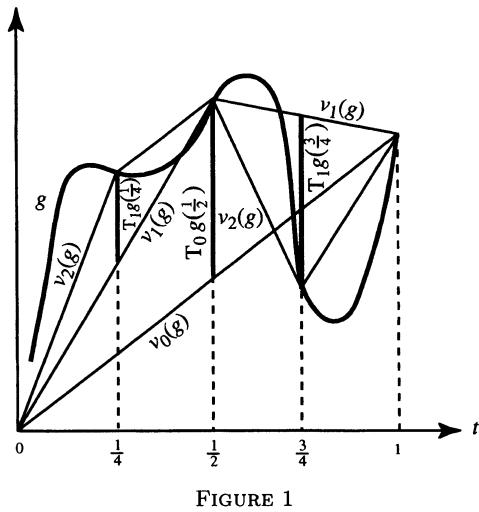
\includegraphics[keepaspectratio]{images/part002_94c2d949.jpg}}

于是可将引理 3 用于 \(t = \frac{k - 1}{2^n}\)、\(t' = \frac{k}{2^n}\)，从而

\[
\int_ {\Omega} \left| \mathrm{T} _ {n} g \left(\frac {2 k - 1}{2 ^ {n + 1}}\right) \right| ^ {3} d m (g) = \frac {1}{(8 \pi) ^ {1 / 2}} 2 ^ {- \frac {3 n}{2}}.\tag{46}
\]

由 (44)，于是有

\[
\int_ {\Omega} \| \mathrm{T} _ {n} g \| ^ {3} d m (g) \leqslant \sum_ {k = 1} ^ {2 ^ {n}} \int_ {\Omega} \left| \mathrm{T} _ {n} g \left(\frac {2 k - 1}{2 ^ {n + 1}}\right) \right| ^ {3} d m (g) = \frac {1}{(8 \pi) ^ {1 / 2}} 2 ^ {n} \cdot 2 ^ {- \frac {3 n}{2}},
\]

因而引理得证。

根据引理 4，从 \(\mathbf{T}_n\)\(\Omega\) 到巴拿赫空间 \(\mathcal{C}\) 的映射  属于 \(\mathrm{L}_{\mathcal{C}}^3 (\Omega ,m)\)，且 \(\mathrm{N}_3(\mathrm{T}_n)\leqslant \frac{1}{(8\pi)^{1 / 6}} (2^{-1 / 6})^n\)，从而 \(\sum_{n = 0}^{\infty}\mathrm{N}_3(\mathrm{T}_n) < + \infty\)。由第 IV 章第 3 节第~3号的命题 6，存在集合 \(\Omega_0\subset \Omega\)，使得 \(\Omega -\Omega_0\) 是 \(m\)-可忽略的，并且对每个 ，级数 \(\sum_{n = 0}^{\infty}\mathrm{T}_n(g)\) 在 \(\mathcal{C}\) 中绝对收敛。于是由下式定义从 \(g\in \Omega_0\)\(m\)\(u\)\(\Omega\) 到 \(\mathcal{C}\) 的 m-可测映射 ：

\[
u (g) = \left\{ \begin{array}{c l} \sum_ {n = 0} ^ {\infty} \mathrm{T} _ {n} g = \lim _ {n \to \infty} u _ {n} (g) & \text { for } g \in \Omega_ {0} \\ 0 & \text { for } g \in \Omega - \Omega_ {0}. \end{array} \right.\tag{47}
\]

由于当  时，\(u_{n}(g)\) 和 g 在 \(g\)\(\mathbf{D}_m \subset \mathbf{D}_n\) 上一致，显然对每个 \(0 \leqslant m \leqslant n\)，\(u(g)\) 在 \(\mathbf{D}\) 上的限制等于 g。\(g\)\(g \in \Omega_0\)

\begin{enumerate}
\def\labelenumi{\Alph{enumi})}
\setcounter{enumi}{2}
\tightlist
\item
  \(\mathcal{C}\) 上的高斯测度的构造：
\end{enumerate}

令 \(w'\) 为 \(\mathcal{C}\) 上的有界测度，它是 m 在 m-可测映射 \(m\)\(m\)\(u: \Omega \to \mathcal{C}\) 下的像。我们将证明 w' 是 \(w'\)\(\mathcal{C}\) 上方差为 W 的高斯测度，从而 w = w'。记 \(W\)\(w = w'\)\(\mathcal{D}\) 为 \(\mathcal{M}^1\) 的线性子空间，它由 t 遍历 D 时的测度 \(\varepsilon_t\) 生成。\(t\)\(D\)

引理 5. --- 对于每个测度 \(\mu \in \mathcal{D}\)，

\[
\int_ {\mathcal {C}} e ^ {i \langle f, \mu \rangle} d w ^ {\prime} (f) = e ^ {- W (\mu) / 2}.\tag{48}
\]

置 \(\mu=c_{1}\varepsilon_{t_{1}}+c_{2}\varepsilon_{t_{2}}+\cdots+c_{n}\varepsilon_{t_{n}}\)，其中 \(t_{1},\ldots,t_{n}\) 属于 D，\(c_{1},\ldots,c_{n}\) 属于 R。对于每个 \(g\in\Omega_{0}\)，函数 \(u(g)\) 在 D 上与 g 一致；因此

\[
\langle u (g), \mu \rangle = \sum_ {j = 1} ^ {n} c _ {j} g (t _ {j}) \quad (g \in \Omega_ {0}).\tag{49}
\]

此外，

\[
\mathrm{W} (\mu) = \sum_ {j, k = 1} ^ {n} c _ {j} c _ {k} \inf (t _ {j}, t _ {k}),\tag{50}
\]

又由于 m 是 \(\Omega\) 上协方差为 M 的高斯测度，且 \(\Omega - \Omega_{0}\) 是 m-可忽略的，有

\[
\int_ {\Omega_ {0}} e ^ {i \sum_ {j = 1} ^ {n} c _ {j} g (t _ {j})} d m (g) = \exp \Big (- \frac {1}{2} \sum_ {j, k = 1} ^ {n} c _ {j} c _ {k} \inf (t _ {j}, t _ {k}) \Big).\tag{51}
\]

现在，\(\Omega - \Omega_0\) 是 \(m\)-可忽略的，且 \(w' = u(m)\)；因此

\[
\int_ {\mathcal {C}} e ^ {i \langle f, \mu \rangle} d w ^ {\prime} (f) = \int_ {\Omega_ {0}} e ^ {i \langle u (g), \mu \rangle} d m (g).\tag{52}
\]

公式 (48) 立即由公式 (49) 至 (52) 得到。

引理 6. --- 设 \(\mu \in \mathcal{M}^1\)。存在测度序列 \(\mu_n \in \mathcal{D}\)，使得对于所有 \(\mu(f) = \lim_{n \to \infty} \mu_n(f)\) 都有 \(f \in \mathcal{C}\)，且 \(\mathrm{W}(\mu) = \lim_{n \to \infty} \mathrm{W}(\mu_n)\)。

令 \(I = [0,1]\)。将 \(\mathcal{M}^1\) 上的有界测度空间 \(T = ]0,1]\) 认作 \(\mathcal{M}(I)\) 的子空间，该子空间由在 0 处不赋予任何权重的测度组成。\(^{(3)}\) 在 \(\mathcal{M}(I)\) 上赋予弱拓扑。映射 \(t \mapsto \varepsilon_t\) 从 I 到 \(\mathcal{M}(I)\) 连续（第 III 章，第 1 节，第~9号，命题 13）；由于 D 在 I 中稠密，\(\overline{\mathcal{D}}\) 的闭包 \(\mathcal{D}\) 包含所有点测度。令 A 为满足 \(\nu \in \mathcal{D}\) 的测度 \(\| \nu \| \leqslant \| \mu \|\) 的集合；测度 \(\mu\) 属于 A 的闭包（第 III 章，第 2 节，第~4号，定理 1 的推论 1）。集合 A 在 \(\mathcal{M}(I)\) 中相对紧（第 III 章，第 1 节，第~9号，命题 15），而 \(\mathcal{M}(I)\) 的紧子集是可度量化的（TVS, III, §3, 第~4号，命题 6 的推论 2，\(^{(4)}\)，以及 GT, X, §3, 第~3号，定理 1）。因此存在测度序列 \(\mu_n \in A\)，在 \(\mu\) 中收敛于 \(\mathcal{M}(I)\)。由于 \(\mathcal{C}\) 可认作 I 上在原点为零的连续函数子空间，对于所有 \(\mu(f) = \lim_{n \to \infty} \mu_n(f)\) 有 \(f \in \mathcal{C}\)。此外，由于 \(\mathcal{C}(I) \otimes \mathcal{C}(I)\) 在赋范空间 \(\mathcal{C}(I \times I)\) 中稠密（第 III 章，第 4 节，第~1号，引理 1），关系 \(\lim_{n \to \infty} \mu_n = \mu\) 和 \(\| \mu_n \| \leqslant \| \mu \|\) 蕴含 \(\lim_{n \to \infty} (\mu_n \otimes \mu_n) = \mu \otimes \mu\)（第 III 章，第 1 节，第~10号，命题 17）；由于测度 \(\mu_n\) 和 \(\mu\) 在 0 处都不赋予权重，有

\[
\begin{array}{r} \mathrm{W} (\mu_ {n}) = \int_ {\mathrm{I}} \int_ {\mathrm{I}} \inf (t, t ^ {\prime}) d \mu_ {n} (t) d \mu_ {n} (t ^ {\prime}), \\ \mathrm{W} (\mu) = \int_ {\mathrm{I}} \int_ {\mathrm{I}} \inf (t, t ^ {\prime}) d \mu (t) d \mu (t ^ {\prime}), \end{array}
\]

从而 \(\lim_{n\to \infty}\mathrm{W}(\mu_n) = \mathrm{W}(\mu)\)。

还需证明 w' 的傅里叶变换等于 \(w'\)\(e^{-\mathbf{W}/2}\)。令 \(\mu \in \mathcal{M}^1\)，按照引理 6 选择测度 \(\mu_n \in \mathcal{D}\)。测度 w' 有界，且对所有 n 都有 \(w'\)\(|e^{i\langle f,\mu_n\rangle}| = 1\)；于是由引理 5 和勒贝格收敛定理（第 IV 章，第 4 节，第~3号，定理 2）可得\(n\)

\[
\begin{array}{r l} \int_ {\mathcal {C}} e ^ {i \langle f, \mu \rangle} d w ^ {\prime} (f) & = \lim _ {n \to \infty} \int_ {\mathcal {C}} e ^ {i \langle f, \mu_ {n} \rangle} d w ^ {\prime} (f) \\ & = \lim _ {n \to \infty} e ^ {- \mathrm{W} (\mu_ {n}) / 2} = e ^ {- \mathrm{W} (\mu) / 2}. \end{array}\tag{Q.E.D.}
\]

傅里叶变换等于 \(w\)\(\mathcal{C}\)\(e^{-\mathrm{W} / 2}\) 的 \(\mathcal{C}\) 上的测度 w 称为  上的维纳测度。

备注. --- 对于 T 中的每个半开区间 \(J = ]a, b]\)，置 \(T\)\(l(J) = b - a\)（J 的长度），并记 \(J\)\(A_J\) 为  上的线性形式 \(f \mapsto f(b) - f(a)\)。可以证明，维纳测度由如下性质刻画：\(\mathcal{C}\)

令 \(J_{1},\ldots,J_{n}\) 是 T 中两两不交的半开区间。测度 w 在从 C 到 \(f\mapsto\left(\mathrm{A}_{\mathrm{J}_{1}}(f),\ldots,\mathrm{A}_{\mathrm{J}_{n}}(f)\right)\) 的线性映射 \(R^{n}\) 下的像等于 \(\gamma_{a_{1}}\otimes\cdots\otimes\gamma_{a_{n}}\)，其中当 \(a_{i}=l(J_{i})^{1/2}\) 时 \(1\leqslant i\leqslant n\)。

\subsection{傅里叶变换的连续性}

命题 8. --- 设 E 是局部凸空间，\(\mu\) 是 E 上的投影测度，\(\Phi\) 是 \(\mu\) 的傅里叶变换。有不等式

\[
\left| \Phi (x ^ {\prime}) \right| \leqslant \Phi (0)\tag{53}
\]

\[
\left| \Phi (x ^ {\prime}) - \Phi (y ^ {\prime}) \right| ^ {2} \leqslant 2 \Phi (0) \big (\Phi (0) - \mathcal {R} \Phi (x ^ {\prime} - y ^ {\prime}) \big)\tag{54}
\]

对于 \(x', y'\) 中的 \(\mathbf{E}'\)。

第~3号的公式 (5) 允许归结为 E 有限维且 \(\mu\) 是测度的情形。于是

\[
\left| \Phi (x ^ {\prime}) \right| = \left| \int_ {\mathrm{E}} e ^ {i \langle x, x ^ {\prime} \rangle} d \mu (x) \right| \leqslant \int_ {\mathrm{E}} | e ^ {i \langle x, x ^ {\prime} \rangle} | d \mu (x) = \int_ {\mathrm{E}} d \mu (x) = \Phi (0),
\]

因此得到 (53)。此外，如果 \(a\) 和 \(b\) 是实数，则

\[
\left| e ^ {i a} - e ^ {i b} \right| ^ {2} = \left| e ^ {i b} \right| ^ {2} \left| e ^ {i (a - b)} - 1 \right| ^ {2} = \left(e ^ {i (a - b)} - 1\right) \left(e ^ {- i (a - b)} - 1\right) = 2 - 2 \cos (a - b);
\]

由柯西--施瓦茨不等式，于是有

\[
\begin{array}{r l} \big | \Phi (x ^ {\prime}) - \Phi (y ^ {\prime}) \big | ^ {2} & = \Big | \int_ {\mathrm{E}} \big (e ^ {i \langle x, x ^ {\prime} \rangle} - e ^ {i \langle x, y ^ {\prime} \rangle} \big) d \mu (x) \Big | ^ {2} \\ & \leqslant \int_ {\mathrm{E}} \big | e ^ {i \langle x, x ^ {\prime} \rangle} - e ^ {i \langle x, y ^ {\prime} \rangle} \big | ^ {2} d \mu (x) \int_ {\mathrm{E}} 1 ^ {2} d \mu (x) \\ & = \int_ {\mathrm{E}} (2 - 2 \cos \langle x, x ^ {\prime} - y ^ {\prime} \rangle) d \mu (x) \cdot \Phi (0) \\ & = 2 \Phi (0) \big (\Phi (0) - \mathcal {R} \Phi (x ^ {\prime} - y ^ {\prime}) \big), \end{array}
\]

因此得到 (54)。

推论. --- 给 E' 赋予一个与其向量空间结构相容的拓扑。Φ 连续的充要条件是其实部 \(\Phi\)\(\mathcal{R}\Phi\) 在原点连续；在此情况下，Φ 一致连续。\(\Phi\)

这由不等式 (54) 得出。

设 F 是局部凸空间。给 F 的对偶 \(F'\) 赋予一个与 F 和 \(F'\) 之间的对偶关系相容的拓扑，并将 F 认作 \(F'\) 的对偶。因此，\(\mu\) 上有界测度 \(F'\) 的傅里叶变换是 F 上的函数 \(F\mu\)，由下式定义

\[
(\mathcal {F} \mu) (x) = \int_ {\mathrm{F} ^ {\prime}} e ^ {i \langle x, x ^ {\prime} \rangle} d \mu (x ^ {\prime}).
\]

命题 9. --- 如果 F 是桶状空间，则 \(F'\) 上每个有界测度的傅里叶变换都是 F 上的一致连续函数。

设 \(\mu\) 是 \(\mathbf{F}'\) 上的有界测度，\(\Phi\) 是其傅里叶变换。令 \(\varepsilon > 0\)。存在  的紧子集 \(\mathbf{K}\)，使得 \(\mathbf{F}'\)\(\mu(\mathbf{F}' - \mathbf{K}) \leqslant \varepsilon\)。现在，\(\mathbf{K}\) 对弱拓扑 \(\sigma(\mathbf{F}', \mathbf{F})\) 是紧的，因而由于 \(\mathbf{F}\) 是桶状空间而等度连续（TVS, III, §4, 第~2号，定理 1）。因此存在  中 0 的对称邻域 \(\mathbf{U}\)，其极集 \(0\)\(\mathbf{F}\)\(\mathbf{U}^{\circ}\) 包含 \(\mathbf{K}\)。令 \(x\)；则\(\varepsilon \mathrm{U}\)

\[
\Phi (0) - \mathcal {R} \Phi (x) = \int_ {\mathrm{F} ^ {\prime}} \left(1 - \cos \langle x, x ^ {\prime} \rangle\right) d \mu (x ^ {\prime}).
\]

现在，\(0 \leqslant 1 - \cos \langle x, x' \rangle \leqslant 2\) 对每个 \(x' \in \mathbf{F}' - \mathbf{K}\)，并且

\[
1 - \cos \langle x, x ^ {\prime} \rangle \leqslant \frac {1}{2} \langle x, x ^ {\prime} \rangle^ {2} \leqslant \frac {\varepsilon^ {2}}{2}
\]

对于 \(x^{\prime}\in \mathbf{K}\subset \mathbf{U}^{\circ}\)；所以

\[
0 \leqslant \Phi (0) - \mathcal {R} \Phi (x) \leqslant 2 \mu (\mathrm{F} ^ {\prime} - \mathrm{K}) + \frac {\varepsilon^ {2}}{2} \mu (\mathrm{K}) \leqslant 2 \varepsilon + \frac {\varepsilon^ {2}}{2} \mu (\mathrm{F} ^ {\prime}).
\]

这个不等式右端随 \(\varepsilon\) 趋于 0；因此 \(\mathcal{R}\Phi\) 在 0 连续，命题由命题 8 的推论得证。

\subsection{Minlos 引理}

设 T 是有限维向量空间，\(\mu\) 是 \(T'\) 上的有界测度；将 T 认作 \(T'\) 的对偶，从而 \(\Phi\) 的傅里叶变换 \(\mu\) 是 T 上的函数。设 T 上给定两个正二次型 h 和 q，以及一个数 \(\varepsilon > 0\)。对于每个实数 r > 0，记 \(C_{r}\) 为满足 \(x' \in T'\)（对所有 \(\langle x, x' \rangle^{2} \leqslant r^{2} h(x)\)）的 \(x \in T\) 的集合。

命题 10. --- 在假设 \(\Phi(0) - \mathcal{R}\Phi \leqslant \varepsilon + q\) 下，有

\[
\mu (\mathrm{T} ^ {\prime} - \mathrm{C} _ {r}) \leqslant 3 \left(\varepsilon + r ^ {- 2} \operatorname{Tr} (q / h)\right)\tag{55}
\]

对于每个 \(r > 0\)。

记 \(\operatorname{Tr}(q/h)\) 为 q 相对于 h 的迹（参见附录，第~1号）。当 \(\operatorname{Tr}(q/h)\) 为无穷时，公式 (55) 是平凡的。以下假设 \(\operatorname{Tr}(q/h)\) 有限，因而对于 \(h(x)=0\)，\(q(x)=0\) 蕴含 \(x\in T\)。

令 \(a_1, \ldots, a_n\) 是 \(\mathbf{T}\) 中的元素，\(\mathbf{D}\) 是满足 \(x' \in \mathbf{T}'\) 的 \(\sum_{j=1}^{n} \langle a_j, x' \rangle^2 > 1\) 的集合。对于每个实数 \(t \geqslant 0\)，有 \(3(1 - e^{-t/2}) \geqslant 0\)，并且还有

\[
3 (1 - e ^ {- t / 2}) \geqslant 3 (1 - e ^ {- 1 / 2}) \geqslant 3 \left(1 - \left(\frac {9}{4}\right) ^ {- 1 / 2}\right) = 1
\]

当 \(t > 1\) 时成立，因为 \(e > \frac{9}{4}\)。将这些不等式用于 \(t = \sum_{j=1}^{n} \langle a_j, x' \rangle^2\)，得到

\[
\mu (\mathrm{D}) \leqslant 3 \int_ {\mathrm{T} ^ {\prime}} \left(1 - \exp \left(- \frac {1}{2} \sum_ {j = 1} ^ {n} \langle a _ {j}, x ^ {\prime} \rangle^ {2}\right)\right) d \mu (x ^ {\prime}).\tag{56}
\]

令 \(\gamma\) 为 \(\mathbf{R}\) 上相对于勒贝格测度密度为 \(t \mapsto (2\pi)^{-1/2} e^{-t^2/2}\) 的测度。由第~4号的引理 2，

\[
\int_ {\mathbf {R}} e ^ {i u t} d \gamma (t) = e ^ {- u ^ {2} / 2}
\]

对于所有实数 \(u\)。因此，

\[
\begin{array}{l} 1 - \exp \left(- \frac {1}{2} \sum_ {j = 1} ^ {n} \langle a _ {j}, x ^ {\prime} \rangle^ {2}\right) \\ = \int \dots \int \left(1 - e ^ {i \sum_ {j = 1} ^ {n} \langle a _ {j}, x ^ {\prime} \rangle t _ {j}}\right) d \gamma (t _ {1}) \dots d \gamma (t _ {n}) \end{array}\tag{57}
\]

对于所有 \(x' \in T'\)。第二成员中关于 \(x', t_{1}, \ldots, t_{n}\) 待积分的函数是连续的，且绝对值有上界 2；而 \(\mu\) 和 \(\gamma\) 都是有界测度。因此可以对 (57) 两端关于 \(d\mu(x')\) 积分，并交换关于 \(\mu\) 和 \(\gamma\) 的积分；得到

\[
\begin{array}{l} \int_ {\mathbf {T} ^ {\prime}} \left(1 - \exp \left(- \frac {1}{2} \sum_ {j = 1} ^ {n} \langle a _ {j}, x ^ {\prime} \rangle^ {2}\right)\right) d \mu (x ^ {\prime}) \\ = \int \dots \int \left(\Phi (0) - \Phi \left(\sum_ {j = 1} ^ {n} t _ {j} a _ {j}\right)\right) d \gamma (t _ {1}) \dots d \gamma (t _ {n}). \end{array}\tag{58}
\]

由于 q 是 \(q\)\(\mathbf{T}\) 上的二次型，存在实数 \(q_{jk}\)，使得

\[
q \left(\sum_ {j = 1} ^ {n} t _ {j} a _ {j}\right) = \sum_ {j, k} q _ {j k} t _ {j} t _ {k}
\]

对于实数 \(t_1, \ldots, t_n\)；特别地，当 \(q_{jj} = q(a_j)\) 时，\(1 \leqslant j \leqslant n\)。此外，积分 \(\int_{\mathbf{R}} t^n d\gamma(t)\) 在 \(n = 0, 1, 2\) 时分别取值 1, 0, 1（第~4号，引理 1）。由此立即得到

\[
\int \dots \int \left(\varepsilon + q \left(\sum_ {j = 1} ^ {n} t _ {j} a _ {j}\right)\right) d \gamma (t _ {1}) \dots d \gamma (t _ {n}) = \varepsilon + \sum_ {j = 1} ^ {n} q (a _ {j}).\tag{59}
\]

现在，(58) 的第一成员和 \(\Phi(0)\) 都是实数；因此可以在 (58) 的第二成员中用 \(\Phi\) 替代 \(R\Phi\)。不等式 \(\Phi(0)-\mathcal{R}\Phi\leqslant\varepsilon+q\) 以及公式 (56)、(58) 和 (59) 蕴含

\[
\mu (\mathrm{D}) \leqslant 3 \left(\varepsilon + \sum_ {j = 1} ^ {n} q (a _ {j})\right).\tag{60}
\]

固定数 \(r > 0\)。由于二次型 h 为正，存在 T 的一个基 \(h\)\((e_1, \ldots, e_n)\) 和一个介于 0 与 n 之间的整数 m，使得\(T\)\(m\)\(n\)

\[
h \left(\sum_ {j = 1} ^ {n} t _ {j} e _ {j}\right) = \sum_ {j = 1} ^ {m} t _ {j} ^ {2}
\]

对于实数 \(t_1, \ldots, t_n\)（附录，第~1号，命题 2）。于是立即可见，\(\mathbf{C}_r\) 由满足下列条件的 \(x' \in \mathbf{T}'\) 组成：

\[
\sum_ {j = 1} ^ {m} \langle e _ {j}, x ^ {\prime} \rangle^ {2} \leqslant r ^ {2}, \quad \sum_ {j = m + 1} ^ {n} \langle e _ {j}, x ^ {\prime} \rangle^ {2} = 0.
\]

对于每个整数 \(l \geqslant 1\)，令 \(D_l\) 为满足下列不等式的 \(x' \in T'\) 的集合

\[
\sum_ {j = 1} ^ {m} \left\langle r ^ {- 1} e _ {j}, x ^ {\prime} \right\rangle^ {2} + \sum_ {j = m + 1} ^ {n} \left\langle l e _ {j}, x ^ {\prime} \right\rangle^ {2} > 1.
\]

容易看出，序列 \((\mathrm{D}_l)_{l\geqslant 1}\) 递增，其并为 \(\mathbf{T}' - \mathbf{C}_r\)，从而

\[
\mu (\mathrm{T} ^ {\prime} - \mathrm{C} _ {r}) = \lim _ {l \to \infty} \mu (\mathrm{D} _ {l}).\tag{61}
\]

但由 (60)，

\[
\mu \left(\mathrm{D} _ {l}\right) \leqslant 3 \left(\varepsilon + \sum_ {j = 1} ^ {m} r ^ {- 2} q \left(e _ {j}\right) + \sum_ {j = m + 1} ^ {n} l ^ {2} q \left(e _ {j}\right)\right);\tag{62}
\]

当 \(j = m + 1, \ldots, n\) 时，有 \(h(e_j) = 0\)，因而 \(q(e_j) = 0\)。此外，\(\operatorname{Tr}(q/h) = \sum_{j=1}^{m} q(e_j)\)（附录，第~1号，命题 2）。关系 (55) 由 (61) 和 (62) 得到。

证毕

\subsection{核空间对偶上的测度}

设 F 是局部凸空间。令 \(T_{s}\) 为弱拓扑 \(\sigma(\mathbf{F}^{\prime},\mathbf{F})\)（定义在 \(F^{\prime}\) 上），令 \(T_{c}\) 为在 F 的紧凸子集上一致收敛的拓扑。根据 Mackey 定理（TVS, IV, §1, 第~1号, 定理 1），\(T_{s}\) 和 \(T_{c}\) 在 \(F^{\prime}\) 上与 F 和 \(F^{\prime}\) 之间的对偶性相容；因此，\(F^{\prime}\) 上每个介于 \(T_{s}\) 与 \(T_{c}\) 之间的局部凸拓扑 T 也具有同样性质。若 T 是这样的拓扑，并且 \(F^{\prime}_{T}\) 表示赋予 T 的 \(F^{\prime}\) 空间，我们将 F 视为 \(F^{\prime}_{T}\) 的对偶。因此，对于上述类型的所有拓扑 T，\(F^{\prime}\) 上的投影测度都相同；若 \(\mu\) 是这样的投影测度，则其傅里叶变换是 F 上的函数。

把 F 上由满足下述条件的连续半范数 N 定义的局部凸拓扑 S 称为萨佐诺夫拓扑：\(N^{2}\) 是 F 上的正二次型，并且存在 F 上的连续正二次型 H，使得 \(\operatorname{Tr}\left(\mathrm{N}^{2}/\mathrm{H}\right)<+\infty\)。拓扑 S 比 F 上给定的拓扑粗；若这两个拓扑相同，则称 F 为核空间。这类空间将在后文详细研究。

定理 2（Minlos）。--- 设 F 是局部凸空间，T 是 \(F'\) 上介于 \(T_{s}\) 与 \(T_{c}\) 之间的局部凸拓扑，\(\mu\) 是 \(F'_{T}\) 上的投影测度。假设  的傅里叶变换 \(\Phi\) 在 F 上关于萨佐诺夫拓扑连续，则 \(\mu\) 是 \(\mu\)\(F'_{T}\) 上的测度。

令 \(\varepsilon > 0\)。由于 \(\Phi\) 在 \(F\) 上关于萨佐诺夫拓扑连续，存在  上的两个连续正二次型 \(Q\) 和 \(H\)，使得 \(F\)\(\operatorname{Tr}(Q / H) < +\infty\)，并且

\[
\Phi (0) - \mathcal {R} \Phi (x) \leqslant \varepsilon / 6
\]

对于每个 \(x \in \mathbf{F}\)（满足 \(\mathbf{Q}(x) \leqslant 1\)），由第~8号命题 8，\(|\mathcal{R}\Phi(x)| \leqslant \Phi(0)\) 对所有 \(x \in \mathbf{F}\) 都成立，因而

\[
\Phi (0) - \mathcal {R} \Phi (x) \leqslant \varepsilon / 6 + 2 \Phi (0) \mathrm{Q} (x)\tag{63}
\]

对于所有 \(x \in \mathbf{F}\) 都成立。

令 \(r = \left(12\Phi(0)\mathrm{Tr}(\mathbf{Q}/\mathbf{H})\varepsilon^{-1}\right)^{1/2}\)，并以 K 表示由满足 \(K\)\(x' \in F_{\mathcal{T}}'\) 且 \(\langle x, x' \rangle^2 \leqslant r^2\mathrm{H}(x)\) 对所有 \(x \in F\) 都成立的元素  构成的集合。由于 \(H^{1/2}\) 是 F 上的连续半范数，集合 K 在 \(F\)\(K\)\(F_{\mathcal{T}}'\) 中等度连续且闭；因此根据 Ascoli 定理（GT, X, §2, 第~5号, 定理 2 的推论 1），它在 \(F_{\mathcal{T}}'\) 中是紧的。

设 V 是 \(F'_{T}\) 的闭线性子空间，且余维有限；则 V 是 F 中某个有限维线性子空间 T 的正交补。令 \(\mu_{V}\) 为 \(T'\) 上的测度，它是  上的投影测度 \(\mu\) 在映射 \(F'_{T}\) 下的像；这里 \(p_{V}\) 是 T 到 F 的典范嵌入的转置；其傅里叶变换是 \(\Phi\) 在 T 上的限制。最后，根据 Hahn--Banach 定理（TVS, II, §3, 第~2号, 定理 1 的推论 1），\(p_{\mathrm{V}}(\mathrm{K})\) 等于集合 \(C_{r}\)，其中 \(x' \in T'\) 由满足 \(\langle x, x' \rangle^{2} \leqslant r^{2}\mathrm{H}(x)\) 对所有 \(x \in T\) 都成立的  构成。由不等式 (63)，可将第~9号命题 10 应用于  上的测度 \(\mu_{V}\)：取 q 为 \(T'\)\(2\Phi(0)\mathrm{Q}\) 在 T 上的限制，取 h 为 H 在 T 上的限制。于是 \(\mathrm{Tr}(q/h) \leqslant 2\Phi(0)\operatorname{Tr}(\mathrm{Q}/\mathrm{H})\)，从而

\[
\mu_ {\mathrm{V}} \left(\mathrm{T} ^ {\prime} - \mathrm{C} _ {r}\right) \leqslant 3 \left(\frac {\varepsilon}{6} + 2 \Phi (0) \operatorname{Tr} (\mathrm{Q} / \mathrm{H}) r ^ {- 2}\right) = \varepsilon .
\]

由于 \(p_V\) 通过取商定义了从 \(F_{\mathcal{T}}' / V\) 到 \(T'\) 的同构，第~1号命题 1 于是表明，\(\mu\) 是 \(F_{\mathcal{T}}'\) 上的测度。

证毕

推论。--- 设 F 是桶状核空间，T 是 \(F'\) 上介于 \(T_{s}\) 与 \(T_{c}\) 之间的局部凸拓扑，\(\mu\) 是 \(F'_{T}\) 上的投影测度，\(\Phi\) 是 \(\mu\) 的傅里叶变换。要使 \(\mu\) 成为测度，\(\Phi\) 在 F 上连续是必要且充分的。

必要性由第~8号命题 9 得出，充分性由定理 2 得出。

备注。--- 设 F 是桶状空间，T 是 \(F'\) 上介于 \(T_s\) 与 \(T_c\) 之间的局部凸拓扑。对于 T，\(F'\) 的每个紧子集在较粗的拓扑 \(T_s\) 下都是紧的。反过来，设 K 是 \(F'\) 的一个在 \(T_s\) 下紧的子集。由于 F 是桶状的，K 是等度连续的（TVS, III, §4, 第~2号, 定理 1）；但根据 Ascoli 定理，\(F'\) 的每个等度连续子集在 \(T_c\) 下相对紧，因而在 T 下更是相对紧的，所以 K 包含于 \(F'\) 的一个在 T 下紧的子集。不难由此推出，从 \(F'_T\) 到 \(F'_{T_s}\) 的恒等映射在这两个空间上的测度集合之间定义了一个双射。

\subsection{希尔伯特空间上的测度}

设 E 是实希尔伯特空间，其内积记作 \((x|y)\)。存在从 E 到其对偶 \(E'\) 的同构 j，由公式 \(\langle x,j(y)\rangle=(x|y)\)（x,y 属于 E）刻画（TVS, V, §1，第~7号，定理 3）。我们借助 j 认同 E 和 \(E'\)。因此，E 上投影测度 \(\mu\) 的傅里叶变换是 E 上的函数 \(\mathcal{F}\mu\)；当 \(\mu\) 是

测度时，有

\[
(\mathcal {F} \mu) (x) = \int_ {\mathrm{E}} e ^ {i (x | y)} d \mu (y) \quad (x \in \mathrm{E}).\tag{64}
\]

定理 3（Prokhorov--Sazonov） --- 设 E 是希尔伯特空间，\(E_{s}\) 是赋予弱化拓扑的空间 E。设 \(\mu\) 是 E 上的投影测度，\(\Phi\) 是其傅里叶变换。下列条件等价：

\begin{enumerate}
\def\labelenumi{\alph{enumi})}
\item
  函数 \(\Phi\) 关于萨佐诺夫拓扑在 \(\mathbf{E}\) 上连续。
\item
  对于每个 \(\varepsilon > 0\)，存在 \(\mathbb{Q}\) 上的核正二次型 \(\mathbf{E}\)，使得 \(\Phi(0) - \mathcal{R}\Phi \leqslant \varepsilon + \mathbb{Q}\)。
\item
  投影测度 \(\mu\) 是 \(\mathbf{E}_s\) 上的测度。
\end{enumerate}

\(b) \Rightarrow a)\)：这由第~8号的命题 8（参见不等式 (54)）得出。

\(a) \Rightarrow c)\)：这由第~10号的定理 2 得出。

\(c) \Rightarrow b)\)：假设 \(\mu\) 是 \(\mathbf{E}_s\) 上的测度。令 \(\varepsilon > 0\)。对于每个整数 \(n \geqslant 1\)，由范数 \(\mathrm{B}_n\) 的 \(x \in \mathbf{E}\) 组成的集合 \(\leqslant n\) 是 \(\mathbf{E}_s\) 的闭子集，且 \(\mathbf{E} = \bigcup_{n \geqslant 1} \mathrm{B}_n\)。因此存在整数 \(n \geqslant 1\)，使得

\(\mu (\mathbf{E} - \mathbf{B}_n) <   \frac{\varepsilon}{2}.\) 该公式

\[
\mathrm{Q} (x) = \frac {1}{2} \int_ {\mathrm{B} _ {n}} (x | y) ^ {2} d \mu (y)\tag{65}
\]

由此在 \(\mathbf{Q}\) 上定义正二次型 \(\mathbf{E}\)。置 \(\mathrm{C} = \frac{n^2}{2}\mu (\mathrm{B}_n)\)。如果 \((e_1,\ldots ,e_p)\) 是 \(\mathbf{E}\) 中的有限正交规范序列，则

\[
\sum_ {j = 1} ^ {p} (e _ {j} | y) ^ {2} \leqslant \| y \| ^ {2} \leqslant n ^ {2}
\]

由 Bessel 不等式，对于每个 \(y \in \mathbf{B}_n\) 都有。积分得到

\[
\sum_ {j = 1} ^ {p} \mathrm{Q} (e _ {j}) = \frac {1}{2} \int_ {\mathrm{B} _ {n}} \sum_ {j = 1} ^ {p} (e _ {j} | y) ^ {2} d \mu (y) \leqslant \frac {n ^ {2}}{2} \mu (\mathrm{B} _ {n}) = \mathrm{C},
\]

因此 Q 是核的。

此外，对于每个实数 \(1 - \cos t \leqslant \inf \left(2, \frac{t^2}{2}\right)\)，有 \(t\)，从而

\[
\begin{array}{r l} \Phi (0) - \mathcal {R} \Phi (x) & = \int_ {\mathrm{E}} \bigl (1 - \cos (x | y) \bigr) d \mu (y) \\ & \leqslant \int_ {\mathrm{B} _ {n}} \frac {1}{2} (x | y) ^ {2} d \mu (y) + \int_ {\mathrm{E} - \mathrm{B} _ {n}} 2 \cdot d \mu (y) \\ & <   \mathrm{Q} (x) + \varepsilon \end{array}
\]

对于所有 \(x \in \mathbf{E}\)。于是 b) 得证。\(b)\)

证毕

推论 1. --- 设 \(E_{1}\) 和 \(E_{2}\) 是两个希尔伯特空间，u 是从 \(E_{1}\) 到 \(E_{2}\) 的希尔伯特--施密特映射，\(\mu\) 是 \(E_{1}\) 上的投影测度。假设 \(\Phi\) 的傅里叶变换 \(\mu\) 在 \(E_{1}\) 上连续。则投影测度 \(\nu = u(\mu)\) 是赋予弱拓扑的 \(E_{2}\) 上的测度。

借助本号中将 \(E_{1}\) 和 \(E_{2}\) 与其对偶作的认同，\(\nu\) 的傅里叶变换等于 \(\Phi\circ u^{*}\)，其中 \(u^{*}\) 是 u 的伴随。现在，\(u^{*}\) 是从 \(E_{2}\) 到 \(E_{1}\) 的希尔伯特--施密特映射（附录，第~2号），所以 \(y\mapsto\|u^{*}(y)\|^{2}\) 上的二次型 \(E_{2}\) 是核的。如果 \((\mathrm{E}_{2})_{\mathcal{S}}\) 表示赋予萨佐诺夫拓扑的 \(E_{2}\)，则 \(u^{*}\) 是从 \((\mathrm{E}_{2})_{\mathcal{S}}\) 到 \(E_{1}\) 的连续线性映射，且 \(\Phi_{\nu}=\Phi\circ u^{*}\) 在 \((\mathrm{E}_{2})_{\mathcal{S}}\) 上连续；于是定理 3 表明，\(\nu\) 是赋予弱拓扑的空间 \(E_{2}\) 上的测度。

推论 2. --- 设 Q 是希尔伯特空间 E 上的核正二次型。E 上方差为 Q 的高斯投影测度 \(\Gamma_{Q}\) 是 \(E_{s}\) 上的测度。

 \(\Phi\)\(\Gamma_{Q}\) 的傅里叶变换等于 \(e^{-\mathbb{Q} / 2}\)。现在，对于每个实数 ，有 \(e^t \geqslant 1 + t\)，从而 \(t\)\(\Phi(0) - \mathcal{R}\Phi \leqslant \mathbb{Q} / 2\)。因此定理 3 的 b) 条件得到验证，\(b)\)\(\Gamma_{Q}\) 是 \(\mathbf{E}_s\) 上的测度。

\subsection{与正型函数的关系}

\begin{enumerate}
\def\labelenumi{(\arabic{enumi})}
\setcounter{enumi}{65}
\tightlist
\item
\end{enumerate}

命题 11. --- 设 E 是有限维向量空间，\(\mu\) 是 E 上的有界（正）测度，\(\Phi\) 是 \(\mu\) 的傅里叶变换。函数 \(\Phi\) 在 \(E'\) 上连续且为正型函数。

由第~8号的命题 9 可得 \(\Phi\) 的连续性。

证明 \(\Phi\) 是正型的。令 \(x_1', \ldots, x_p'\) 属于 E'，\(c_1, \ldots, c_p\) 为复数。则

\[
\begin{array}{r l} \sum_ {j, k} c _ {j} \overline {{{c}}} _ {k} \Phi (x _ {j} ^ {\prime} - x _ {k} ^ {\prime}) & = \int_ {\mathrm{E}} \sum_ {j, k} c _ {j} \overline {{{c}}} _ {k} e ^ {i \langle x, x _ {j} ^ {\prime} - x _ {k} ^ {\prime} \rangle} d \mu (x) \\ & = \int_ {\mathrm{E}} \left| \sum_ {j = 1} ^ {p} c _ {j} e ^ {i \langle x, x _ {j} ^ {\prime} \rangle} \right| ^ {2} d \mu (x) \geqslant 0. \end{array}\tag{Q.E.D.}
\]

可以证明一个称为博赫纳定理的逆命题：\(E'\) 上每个连续的正型函数都是某个有界（正）测度的傅里叶变换。\(^{*}\) 在第~12号余下部分假设这一结果成立。

定理 4. --- 设 E 是局部凸空间。傅里叶变换是从 E 上的投影测度集合到  上正型函数集合的双射，其中后者的函数限制在每个有限维子空间上都连续。

我们知道（第~3号的命题 3），傅里叶变换是单射。令 \(\mu = (\mu_{\mathrm{V}})_{\mathrm{V}\in \mathcal{F}(\mathbf{E})}\) 是 \(\mathbf{E}\) 上的投影测度，\(\Phi\) 是其傅里叶变换。令 \(\mathbf{T}\) 是 \(\mathbf{E}'\) 的有限维子空间，\(\mathbf{V}\) 是 \(\mathbf{T}\) 中 \(\mathbf{E}\) 的正交补。可将 \(\mathbf{T}\) 认作 \(\mathbf{E} / \mathbf{V}\) 的对偶；\(\Phi_{\mathrm{T}}\) 是 \(\Phi\) 在 \(\mathbf{T}\) 上的限制，也是 \(\mu_{\mathrm{V}}\) 上有界测度 \(\mathbf{E} / \mathbf{V}\) 的傅里叶变换。由命题 11，\(\Phi_{\mathrm{T}}\) 在 \(\mathbf{T}\) 上连续且为正型。由于 \(\mathbf{T}\) 任意，显然 \(\Phi\) 在 \(\mathbf{E}'\) 上为正型。

反过来，令 \(\Phi\) 是 \(\mathbf{E}'\) 上的正型函数，且其限制在 \(\mathbf{E}'\) 的每个有限维子空间上都连续。对于每个 \(V \in \mathcal{F}(\mathbf{E})\)，将 E/V 的对偶认作 \(E/V\) 中 V 的正交补 \(V^{\circ}\)；\(V\)\(\mathbf{E}'\)\(\Phi_V\) 是 \(\Phi\) 在 \(V^{\circ}\) 上的限制，它连续且为正型，因此由博赫纳定理，存在 E/V 上的有界（正）测度 \(\mu_V\)，其傅里叶变换为 \(E/V\)\(\Phi_V\)。设 \(V\) 和 \(W\) 属于 \(\mathcal{F}(\mathbf{E})\) 且 \(W \subset V\)，并令 \(p_{\mathrm{VW}}\) 为从 E/W 到 E/V 的典范映射；在上述认同下，\(E/W\)\(E/V\)\(^{t}p_{\mathrm{VW}}\) 是从 \(V^{\circ}\) 到 \(W^{\circ}\) 的嵌入。由第~3号的公式 (4)，于是有

\[
\mathcal {F} \big (p _ {\mathrm{VW}} (\mu_ {\mathrm{W}}) \big) = \big (\mathcal {F} \mu_ {\mathrm{W}} \big) \circ {} ^ {t} p _ {\mathrm{VW}} = \Phi_ {\mathrm{W}} \circ {} ^ {t} p _ {\mathrm{VW}} = \Phi_ {\mathrm{V}} = \mathcal {F} \mu_ {\mathrm{V}},
\]

因此由第~3号的命题 3，\(p_{\mathrm{VW}}(\mu_{\mathrm{W}}) = \mu_{\mathrm{V}}\)。所以族 \(\mu = (\mu_{\mathrm{V}})_{\mathrm{V} \in \mathcal{F}(\mathrm{E})}\) 是 E 上的投影测度；显然 \(\Phi\) 是 \(\mu\) 的傅里叶变换。

推论. --- 设 F 是桶状核空间；给 \(F'\) 赋予局部凸拓扑 T，使其介于弱拓扑 \(\sigma(\mathbf{F}',\mathbf{F})\) 与 F 的紧凸子集上的一致收敛拓扑之间。傅里叶变换是从 \(F'\) 上的有界（正）测度集合到 F 上连续正型函数集合的双射。

这立即由第 4 号定理和第~10号定理 2 的推论得出。*

\specsection{附录：希尔伯特空间补充}

\annexsubsection{\texorpdfstring{关于另一个二次型的二次型的迹 \(^{(1)}\)}{关于另一个二次型的二次型的迹 (1)}}

在本号中，记 E 为实向量空间，Q、H 为 E 上的两个正二次型。存在两个对称双线性型 \((x,y)\mapsto(x|y)_{\mathbf{Q}}\) 和 \((x,y)\mapsto(x|y)_{\mathbf{H}}\)，由下式刻画

\[
\mathrm{Q} (x) = (x | x) _ {\mathrm{Q}}, \quad \mathrm{H} (x) = (x | x) _ {\mathrm{H}}
\]

对于所有 \(x \in E\)。

称 Q 关于 H 的迹，并用 \(\operatorname{Tr}\left(\mathbf{Q}/\mathbf{H}\right)\) 表示如下定义的、可能有限也可能不有限的正实数：

\begin{enumerate}
\def\labelenumi{\alph{enumi})}
\item
  如果存在 \(x \in \mathbf{E}\)，使得 \(\mathrm{H}(x) = 0\) 且 \(\mathrm{Q}(x) \neq 0\)，则置 \(\operatorname{Tr}(\mathrm{Q} / \mathrm{H}) = +\infty\)。
\item
  在相反情况下，\(\operatorname{Tr}(\mathbf{Q}/\mathbf{H})\) 是形如 \(\sum_{i=1}^{p} \mathbf{Q}(e_i)\) 的数的集合的上确界，其中 \((e_1, \ldots, e_p)\) 遍历 E 中关于 H 正交规范的有限序列。
\end{enumerate}

设 E 是实希尔伯特空间，Q 是 E 上的正二次型。对所有 \(\mathrm{H}(x)=\|x\|^{2}\) 置 \(x\in E\)；于是 H 是 E 上的正二次型。如果 \(\mathrm{Tr}\left(\mathrm{Q}/\mathrm{H}\right)\) 有限，则称 Q 是核的。对于 E 中每个范数为 1 的 \(x\in E\)，有 \(\mathrm{Q}(x)\leqslant\mathrm{Tr}\left(\mathrm{Q}/\mathrm{H}\right)\)，从而 \(Q\leqslant\mathrm{Tr}\left(\mathrm{Q}/\mathrm{H}\right)\cdot\mathrm{H}\)；特别地，每个核型 Q 都连续。

备注. --- 1) 对于 E 的每个子空间 F，记 \(Q_{F}\) 为 Q 在 F 上的限制，记 \(H_{F}\) 为 H 在 F 上的限制。则 \(\mathrm{Tr}\left(\mathrm{Q}_{\mathrm{F}}/\mathrm{H}_{\mathrm{F}}\right) \leqslant \mathrm{Tr}\left(\mathrm{Q}/\mathrm{H}\right)\)，且 \(\mathrm{Tr}\left(\mathrm{Q}/\mathrm{H}\right)\) 是 \(\mathrm{Tr}\left(\mathrm{Q}_{\mathrm{F}}/\mathrm{H}_{\mathrm{F}}\right)\) 为有限维时各数 \(F \subset E\) 的上确界。

\begin{enumerate}
\def\labelenumi{\arabic{enumi})}
\setcounter{enumi}{1}
\tightlist
\item
  设 \(\mathbf{E}_1\) 是实向量空间，\(\mathbf{Q}_1\) 和 \(\mathbf{H}_1\) 是 \(\mathbf{E}_1\) 上的两个正二次型，\(\pi: \mathbf{E} \to \mathbf{E}_1\) 是满射线性映射。如果 \(\mathbf{Q} = \mathbf{Q}_1 \circ \pi\) 且 \(\mathbf{H} = \mathbf{H}_1 \circ \pi\)，则 \(\operatorname{Tr}(\mathbf{Q} / \mathbf{H}) = \operatorname{Tr}(\mathbf{Q}_1 / \mathbf{H}_1)\)。
\end{enumerate}

命题 1. --- 假设 E 是有限维的，且 H 非退化。

\begin{enumerate}
\def\labelenumi{\alph{enumi})}
\item
  存在  的自同态 \(u\)，由 （x, y 属于 \(\mathbf{E}\)）刻画。\((x|y)_{\mathbb{Q}} = (u(x)|y)_{\mathbb{H}}\)\(x, y\)\(\mathbf{E}\)
\item
  \(\operatorname{Tr}(\mathbf{Q} / \mathbf{H}) = \operatorname{Tr}(u)\)。
\item
  \(\operatorname{Tr}(\mathbf{Q} / \mathbf{H}) = \sum_{i=1}^{m} \mathbf{Q}(e_i)\)，其中 \((e_1, \ldots, e_m)\) 是 E 的任意关于 H 正交规范的基。
\end{enumerate}

 a) 由双线性型 \((x,y)\mapsto (x|y)_{\mathrm{H}}\) 非退化这一事实得到。E 中关于 H 正交规范的每个序列都可以补成 E 的关于 H 正交规范的一个基。因此，\(\operatorname {Tr}(\mathbf{Q} / \mathbf{H})\) 是 \(\sum_{i = 1}^{m}\mathbf{Q}(e_i)\) 形式的数在 E 的所有关于 H 正交规范的基 \((e_1,\ldots ,e_m)\) 上所成集合的上确界。要证明 b) 和 c)，只需证明对于每个这种基都有 \(\sum_{i = 1}^{m}\mathbf{Q}(e_i) =\) \(\operatorname {Tr}(u)\)。对于 \(a_{ij} = (u(e_i)|e_j)_{\mathrm{H}} = (e_i|e_j)_{\mathrm{Q}}\)，置 \(1\leqslant i,j\leqslant m\)；于是当 \(u(e_i) = \sum_{j = 1}^{m}a_{ij}e_j\) 时，\(1\leqslant i\leqslant m\)，从而

\[
\operatorname{Tr} (u) = \sum_ {i = 1} ^ {m} a _ {i i} = \sum_ {i = 1} ^ {m} \left(e _ {i} \mid e _ {i}\right) _ {\mathrm{Q}} = \sum_ {i = 1} ^ {m} Q \left(e _ {i}\right).\tag{Q.E.D.}
\]

命题 2. --- 假设 E 是有限维的。存在 E 的一个基 \((e_{1},\ldots,e_{n})\) 和一个满足 \(0\leqslant m\leqslant n\) 的整数 m，使得

\[
\mathrm{H} \left(\sum_ {i = 1} ^ {n} t _ {i} e _ {i}\right) = \sum_ {i = 1} ^ {m} t _ {i} ^ {2}\tag{1}
\]

对于实数 \(t_1, \ldots, t_n\)。此外，如果对于 \(\mathrm{H}(x) = 0\)，关系 \(\mathrm{Q}(x) = 0\) 蕴含 \(x \in \mathbf{E}\)，则 \(\operatorname{Tr}(\mathrm{Q}/\mathrm{H}) = \sum_{i=1}^{m} \mathrm{Q}(e_i)\)。

存在 E 的一个关于 H 正交的基 \((e_1', \ldots, e_n')\)。可以假定对基编号的方式使得当 \(\mathrm{H}(e_i') > 0\) 时 \(1 \leqslant i \leqslant m\)，而当 \(\mathrm{H}(e_i') = 0\) 时 \(m < i \leqslant n\)。于是，当 \(e_i = e_i' / \mathrm{H}(e_i')^{1/2}\) 时置 \(1 \leqslant i \leqslant m\)，当 \(e_i = e_i'\) 时置 \(m < i \leqslant n\)；关系 (1) 得到满足。

令 F 为由 \(e_{m+1}^{\prime},\ldots,e_{n}^{\prime}\) 生成的 E 的子空间；它正是满足 \(x\in E\) 的 \(\mathrm{H}(x)=0\) 的集合。记 \(\pi\) 为从 E 到 \(E_{1}=E/F\) 的典范映射。由于 Q 和 H 在 F 上为零，存在 \(Q_{1}\) 上的两个正二次型 \(H_{1}\) 和 \(E_{1}\)，使得 \(Q=Q_{1}\circ\pi\) 且 \(H=H_{1}\circ\pi\)。此外，\((\pi(e_{1}),\ldots,\pi(e_{m}))\) 是 \(E_{1}\) 的关于 \(H_{1}\) 正交规范的基，因而 \(H_{1}\) 非退化。

由命题 1 和备注 2，

\[
\operatorname{Tr} \left(\mathrm{Q} / \mathrm{H}\right) = \operatorname{Tr} \left(\mathrm{Q} _ {1} / \mathrm{H} _ {1}\right) = \sum_ {i = 1} ^ {m} \mathrm{Q} _ {1} \left(\pi (e _ {i})\right) = \sum_ {i = 1} ^ {m} \mathrm{Q} (e _ {i}).\tag{Q.E.D.}
\]

备注 3). --- 假设 E 有限维且 H 非退化。设 \((e_1, \ldots, e_n)\) 是 E 的一个基。置 \(q = ((e_i | e_j)_Q)_{1 \leqslant i, j \leqslant n}\)，\(h = ((e_i | e_j)_H)_{1 \leqslant i, j \leqslant n}\)。用命题 1 中的记号，u 关于 E 的基 \(u\)\((e_1, \ldots, e_n)\) 的矩阵等于 \(h^{-1}q\)，从而

\[
\operatorname{Tr} \left(\mathrm{Q} / \mathrm{H}\right) = \operatorname{Tr} \left(h ^ {- 1} q\right) = \operatorname{Tr} \left(q h ^ {- 1}\right).\tag{2}
\]

\annexsubsection{\texorpdfstring{希尔伯特--施密特映射 \(^{(2)}\)}{希尔伯特--施密特映射 (2)}}

设 E 是实希尔伯特空间，内积记作 \((x|y)\)。存在从 E 到其对偶的等距同构 \(j_{E}\)，由下式刻画

\[
(x | y) = \langle x, j _ {\mathrm{E}} (y) \rangle \quad \text { for } x, y \text { in } \mathrm{E}\tag{3}
\]

（TVS, V, §1，第~7号，定理 3）。

设 \(E_{1}\) 和 \(E_{2}\) 是两个实希尔伯特空间，u 是从 \(E_{1}\) 到 \(E_{2}\) 的连续线性映射。将从 \(u^{*} = j_{E_{1}}^{-1} \circ {}^{t}u \circ j_{E_{2}}\) 到 \(E_{2}\) 的连续线性映射 \(E_{1}\) 称为 u 的伴随。映射 \(u^{*}\) 由关系刻画

\[
(u (x _ {1}) | x _ {2}) = (x _ {1} | u ^ {*} (x _ {2})) \quad \text { for } x _ {1} \in \mathrm{E} _ {1}, x _ {2} \in \mathrm{E} _ {2}.\tag{4}
\]

如果 \(v\) 是从 \(\mathbf{E}_2\) 到希尔伯特空间 \(\mathbf{E}_3\) 的连续线性映射，则 \((v \circ u)^* = u^* \circ v^*\)。

设 \(E_{1}\) 和 \(E_{2}\) 是两个实希尔伯特空间，u 是从 \(E_{1}\) 到 \(E_{2}\) 的线性映射。由下列公式在 \(E_{1}\) 上定义两个正二次型 H 和 Q

\[
\mathrm{H} (x) = \| x \| ^ {2}, \quad \mathrm{Q} (x) = \| u (x) \| ^ {2} \qquad (x \in \mathrm{E} _ {1}).
\]

命题 3. --- 假设 u 连续。令 \((e_{i})_{i\in I}\) 是 \(E_{1}\) 的正交规范基，\((f_{j})_{j\in J}\) 是 \(E_{2}\) 的正交规范基。则

\[
\operatorname{Tr} (\mathrm{Q} | \mathrm{H}) = \sum_ {i \in \mathrm{I}} \| u (e _ {i}) \| ^ {2} = \sum_ {j \in \mathrm{J}} \| u ^ {*} (f _ {j}) \| ^ {2} = \sum_ {i \in \mathrm{I}} \sum_ {j \in \mathrm{J}} (u (e _ {i}) | f _ {j}) ^ {2}.
\]

对于每个 \(x \in \mathbf{E}_1\)，有 \(\|x\|^2 = \sum_{i \in \mathbf{I}} (x|e_i)^2\)；类似地，对于每个 \(\|y\|^2 = \sum_{j \in \mathbf{J}} (y|f_j)^2\)，有 \(y \in \mathbf{E}_2\)。因此

\[
\begin{array}{r l} \sum_ {i \in \mathrm{I}} \| u (e _ {i}) \| ^ {2} & = \sum_ {i \in \mathrm{I}} \sum_ {j \in \mathrm{J}} (u (e _ {i}) | f _ {j}) ^ {2} \\ & = \sum_ {j \in \mathrm{J}} \sum_ {i \in \mathrm{I}} (e _ {i} | u ^ {*} (f _ {j})) ^ {2} \\ & = \sum_ {j \in \mathrm{J}} \| u ^ {*} (f _ {j}) \| ^ {2}. \end{array}
\]

特别地，数 \(\sum_{i\in I}\| u(e_i)\|^2\) 与 \((e_i)_{i\in I}\) 的正交规范基 \(\mathbf{E}_1\) 的选取无关。

置 \(t = \operatorname{Tr}(\mathbf{Q}|\mathbf{H})\)。按照定义，对于 I 的每个有限子集 \(I'\)，\(I\)

\[
\sum_ {i \in I ^ {\prime}} \| u (e _ {i}) \| ^ {2} = \sum_ {i \in I ^ {\prime}} Q (e _ {i}) \leqslant t,
\]

从而 \(\sum_{i\in I}\| u(e_i)\|^2\leqslant t\)。令 \((e_1',\dots ,e_p')\) 是 \(\mathbf{E}_1\) 中的有限正交规范序列。该序列可以补成 \((e_{\alpha}^{\prime})_{\alpha \in A}\) 的正交规范基 \(\mathbf{E}_1\)。于是

\[
\sum_ {\alpha = 1} ^ {p} \left\| u (e _ {\alpha} ^ {\prime}) \right\| ^ {2} \leqslant \sum_ {\alpha \in \mathrm{A}} \left\| u (e _ {\alpha} ^ {\prime}) \right\| ^ {2} = \sum_ {i \in \mathrm{I}} \left\| u (e _ {i}) \right\| ^ {2}
\]

对所有 \((e_1', \ldots, e_p')\) 取上确界，得到不等式 \(t \leqslant \sum_{i \in I} \| u(e_i) \|^2\)。从而已证明等式 \(t = \sum_{i \in I} \| u(e_i) \|^2\)。

证毕

如果 \(u\) 上的正二次型  是核的，则称 u 是从 \(\mathbf{E}_1\) 到 \(\mathbf{E}_2\) 的希尔伯特--施密特映射。在此情况下，有 \(\mathbf{Q}: x \mapsto \| u(x) \|^2\)\(\mathbf{E}_1\)\(\mathbf{Q} \leqslant \operatorname{Tr}(\mathbf{Q}/\mathbf{H}) \cdot \mathbf{H}\)，因此 u 连续且\(u\)

\[
\| u \| \leqslant \operatorname{Tr} (\mathrm{Q/H}) ^ {1 / 2}.
\]

设 \(u: \mathbf{E}_1 \to \mathbf{E}_2\) 是连续线性映射。由命题 3，u 是希尔伯特--施密特映射，当且仅当存在 \(u\) 的正交规范基 \((e_i)_{i \in \mathrm{I}}\)，使得 \(\mathbf{E}_1\)\(\sum_{i \in \mathrm{I}} \|u(e_i)\|^2 < +\infty\)。在此情况下，\(\mathbf{E}_1\) 的每个正交规范基都具有同一性质。此外，如果 u 是希尔伯特--施密特映射，则由公式 \(u\)（命题 3），其伴随 \(u^*\) 也是希尔伯特--施密特映射。\(\sum_{i \in \mathrm{I}} \|u(e_i)\|^2 = \sum_{j \in \mathrm{J}} \|u^*(f_j)\|^2\)

\specialchapter{习题}

\exercisesection{}

\begin{enumerate}
\def\labelenumi{\arabic{enumi})}
\tightlist
\item
  设 \(\mathbf{T}\) 是一个集合，\(p\) 是 \(\mathbf{T}\) 上的负荷。对于 \(\mathbf{A}\) 的每个子集 \(\mathbf{T}\)，置 \(p(\mathbf{A}) = p(\varphi_{\mathbf{A}})\)。
\end{enumerate}

\begin{enumerate}
\def\labelenumi{\alph{enumi})}
\item
  当 A 包含于 B 时，\(p(A) \leqslant p(B)\)。
\item
  对于 \((\mathbf{A}_n)\) 的任意有限或无限子集序列 \(\mathbf{T}\)，有 \(p(\bigcup \mathbf{A}_n) \leqslant \sum p(\mathbf{A}_n)\)。
\item
  对于 T 的任意递增子集序列 \((\mathrm{A}_n)_{n\geqslant 1}\)，有 \(p\big(\bigcup_{n}\mathrm{A}_{n}\big) = \lim_{n\to \infty}p(\mathrm{A}_n)\)。
\end{enumerate}

\begin{enumerate}
\def\labelenumi{\arabic{enumi})}
\setcounter{enumi}{1}
\tightlist
\item
  设 \(\mathbf{T}\) 是一个集合，\(p\) 是 \(\mathbf{T}\) 上的负荷。如果 \(f \in \mathcal{F}_{+}(\mathbf{T})\)（分别地，如果 A 是 \(\mathbf{T}\) 的子集），且 \(p\)（分别地，\(p(f) = 0\)），则称 f（分别称 A）为 \(p(\mathbf{A}) = 0\)-可忽略的。
\end{enumerate}

\begin{enumerate}
\def\labelenumi{\alph{enumi})}
\item
  设 \(f\) 和 \(g\) 属于 \(\mathcal{F}_{+}(\mathrm{T})\)，且 t 是满足 \(t\)\(f \leqslant t \cdot g\) 的正实数。若 g 是 \(g\)\(p\)\(f\)\(p\)-可忽略的，则 f 也是如此。\(p\)-可忽略函数序列的和与上包络也是 -可忽略的。
\item
  \(p\)-可忽略集的每个子集都是 \(p\)-可忽略的，\(p\)-可忽略集的有限或无限序列的并也是如此。
\item
  设 \(f \in \mathcal{F}_+(\mathrm{T})\)。对于每个有限实数 \(a > 0\)，记 \(\mathbf{T}_a\) 为满足  的 \(t \in \mathrm{T}\) 的集合。证明 \(f(t) \geqslant a\)\(p(\mathbf{T}_a) \leqslant a^{-1} \cdot p(f)\)。由此推出，f 是 \(f\)\(p\)-可忽略的，当且仅当满足  的 \(t \in \mathrm{T}\) 的集合是 \(f(t) \neq 0\)\(p\)-可忽略的。
\item
  设 \(f \in \mathcal{F}_{+}(\mathrm{T})\)。如果 \(p(f)\) 有限，则满足 f(t) 为无穷的 \(t \in \mathrm{T}\) 的集合是 \(f(t)\)\(p\)-可忽略的。
\item
  设 \(f\) 和 \(g\) 属于 \(\mathcal{F}_{+}(\mathrm{T})\)。如果满足 \(t \in \mathrm{T}\) 的 \(f(t) \neq g(t)\) 的集合是 \(p\)-可忽略的，则 \(p(f) = p(g)\)。
\end{enumerate}

\begin{enumerate}
\def\labelenumi{\arabic{enumi})}
\setcounter{enumi}{2}
\item
  设 \(\mathbf{T}\) 是一个集合，\(p\) 是 \(\mathbf{T}\) 上的负荷。对于 \((f_n)_{n\geqslant 1}\) 中元素的每个序列 \(\mathcal{F}_{+}(\mathbf{T})\)，有 \(p(\liminf_{n\to \infty}f_n)\leqslant \liminf_{n\to \infty}p(f_n)\)。
\item
  设 \(\mathbf{T}\) 是一个集合，\(\mathbf{M}\) 是 \(\mathbf{T}\) 上的负荷，\(\mathbf{E}\) 是实或复巴拿赫空间，p 是满足 \(p\)\(p \geqslant 1\) 的有限实数。记 \(\mathcal{F}\) 为从 \(\mathbf{T}\) 到 \(\mathbf{E}\) 的映射集合，并且对于 \(f\)\(\mathcal{F}\) 或 \(\mathcal{F}_{+}(\mathbf{T})\) 中的 f，置 \(\mathrm{N}_p(f) = \mathrm{M}(|f|^p)^{1/p}\)。
\end{enumerate}

\begin{enumerate}
\def\labelenumi{\alph{enumi})}
\item
  对于 \((f_n)_{n\geqslant 1}\) 中元素的每个序列 \(\mathcal{F}_{+}(\mathrm{T})\)，有 \(\mathrm{N}_p\left(\sum_{n\geqslant 1}f_n\right)\leqslant \sum_{n\geqslant 1}\mathrm{N}_p(f_n)\)
\item
  令 \(\mathcal{F}^p\) 为满足 \(f \in \mathcal{F}\) 有限的 \(\mathrm{N}_p(f)\) 的集合。证明 \(\mathcal{F}^p\) 是 \(\mathcal{F}\) 的线性子空间，\(\mathrm{N}_p\) 是 \(\mathcal{F}^p\) 上的半范数。证明，满足 \(\mathcal{N}\) 的 \(f \in \mathcal{F}^p\) 所成的集合 \(\mathrm{N}_p(f) = 0\)，等于在某个 M-可忽略集之外为零的 \(f \in \mathcal{F}\) 所成的集合。证明赋范空间 \(\mathcal{F}^p / \mathcal{N}\) 是完备的（参见第 IV 章，第 3 节，第~3号）。
\end{enumerate}

\begin{enumerate}
\def\labelenumi{\arabic{enumi})}
\setcounter{enumi}{4}
\item
  设 \(\mathbf{T}\) 是一个集合。记 \(\mathcal{B}_{+}(\mathbf{T})\) 为 \(\mathbf{T}\) 上有界正实函数的集合，记 \(p_0\) 为从 \(\mathcal{B}_{+}(\mathbf{T})\) 到  的区间 \([0, +\infty]\) 的映射，它满足第~1号定义 1 的条件 a) 至 d)。对于每个函数 \(\overline{\mathbf{R}}\)\(a)\)\(d)\)\(f \in \mathcal{F}_{+}(\mathbf{T})\)，记 \(p(f)\) 为数集 \(p_0(f_0)\) 的上确界，其中 \(f_0\) 遍历所有满足 \(\leqslant f\) 的有界函数。证明 p 是 \(p\)\(\mathbf{T}\) 上的负荷。将 \(\mathcal{B}_{+}(\mathbf{T})\) 换成 \(\mathbf{T}\) 上（有限）正实函数的集合后，问题同样成立。
\item
  设 \(\mathbf{T}\) 是一个集合，\(\mathcal{I}_{+}\) 是 \(\mathcal{F}_{+}(\mathrm{T})\) 的子集，\(\mathbf{M}\) 是从 \(\mathcal{I}_{+}\) 到 \(\overline{\mathbf{R}}_{+}\) 的映射。作如下假设：
\end{enumerate}

\begin{enumerate}
\def\labelenumi{\alph{enumi})}
\item
  对于每个 \(f \in \mathcal{I}_+\) 和每个实数 \(t \geqslant 0\)，函数 \(t \cdot f\) 属于 \(\mathcal{I}_+\)，且 \(M(t \cdot f) = t \cdot M(f)\)。
\item
  如果 f 和 g 属于 \(f\)\(g\)\(\mathcal{I}_+\)，那么 \(f + g\)、\(\sup(f, g)\) 和 \(\inf(f, g)\) 也属于 ，且有 \(M(f + g) = M(f) + M(g)\)。
\item
  对于 \((f_n)_{n\geqslant 1}\) 中元素的每个递增序列 \(\mathcal{I}_+\)，函数 \(f = \sup f_n\) 属于 \(\mathcal{I}_+\)，且 \(\mathrm{M}(f) = \lim_{n\to \infty}\mathrm{M}(f_n)\)。
\end{enumerate}

对于每个函数 \(f \in \mathcal{F}_{+}(\mathrm{T})\)，置 \(p(f) = \inf_{g \in \mathcal{I}_{+}, g \geqslant f} \mathrm{M}(g)\)。证明 p 是 \(p\)\(\mathrm{T}\) 上的负荷（参见第 IV 章，第 1 节，第~3号）。如果 f 和 g 属于 \(f\)\(g\)\(\mathcal{F}_{+}(\mathrm{T})\)，且 \(\mathrm{A}\) 和 \(\mathrm{B}\) 是 \(\mathrm{T}\) 的子集，则 \(p(\sup(f, g)) + p(\inf(f, g)) \leqslant p(f) + p(g)\)，并且 \(p(\mathrm{A} \cup \mathrm{B}) + p(\mathrm{A} \cap \mathrm{B}) \leqslant p(\mathrm{A}) + p(\mathrm{B})\)。

\begin{enumerate}
\def\labelenumi{\arabic{enumi})}
\setcounter{enumi}{6}
\tightlist
\item
  在 Lindelöf 空间上，每个测度、每个函数和每个子集都是可控的。
\end{enumerate}

¶ 8) 再次使用第 IV 章第 1 节习题 5 的记号。回忆 \(\mu = \sum_{k=-\infty}^{\infty} \sum_{n=1}^{\infty} n^{-3} \varepsilon_{(1/n,k/n^2)}\)，且 \(\mu^{*}(D) = +\infty\)。证明 \(\mu^{\bullet}(D) = 0\)；由此推出 \(\mu\) 不是可控的，尽管它是具有两两不交紧支集的测度级数之和。证明存在将 X 划分为 Borel 子集  的划分 \((X_n)_{n \in \mathbb{N}}\)，使得对于每个 \(X\)，\(X_n\)\(\mu^{\bullet}(X_n)\) 都有限。\(n \in \mathbb{N}\)

\begin{enumerate}
\def\labelenumi{\arabic{enumi})}
\setcounter{enumi}{8}
\item
  设 \(\mathbf{T}\) 是拓扑空间。如果 \(\lambda\) 和 \(\mu\) 是 \(\mathbf{T}\) 上的两个正测度，且对于 \(\lambda^{\bullet}(\mathrm{U}) = \mu^{\bullet}(\mathrm{U})\) 中的每个开集 \(\mathbf{U}\) 都有 \(\mathbf{T}\)，则 \(\lambda = \mu\)（先证明对于 \(\lambda^{\bullet}(f) = \mu^{\bullet}(f)\) 上每个满足 \(f \geqslant 0\) 的下半连续函数 f，都有 \(\mathbf{T}\)，再证明 \(\lambda^{\bullet} = \mu^{\bullet}\)）。
\item
  设 \(\mathbf{T}\) 是拓扑空间，\(\mu\) 是 \(\mathbf{T}\) 上的正测度；假设 \(\mathbf{T}\) 是一列 \(\mu\)-可积集 \(\mathbf{T}_n\)（\(n \geqslant 0\)）的并。记 \(\mathfrak{C}\) 为由紧子集生成的 \(\mathbf{T}\) 的子集族。
\end{enumerate}

\begin{enumerate}
\def\labelenumi{\alph{enumi})}
\item
  设 X 是 Lusin 空间。对于每个从 T 到 X 的 \(\mu\)-可测映射 f，存在映射序列 \(f\)\(f_m: \mathrm{T} \to \mathrm{X}\)，具有如下性质：\(\alpha\)：对于 \(\mu\)-几乎处处的 \(t \in \mathrm{T}\)，\(f(t) = \lim_{m \to \infty} f_m(t)\)；\(\beta\)：对于每个整数 m，存在将 T 划分为 \(m\)\(\mathrm{A}_j \in \mathfrak{C}\) 的有限划分，使得 \(f_m\) 在每个 \(\mathrm{A}_j\) 上为常值（化归到 \(\mathrm{T}_n\) 构成 T 的一个划分、\(\mathrm{T}_0\) 是 \(\mu\)-可忽略的、当  时 \(\mathrm{T}_n\) 是紧的且 X 是 Polish 空间的情形）。\(n \geqslant 1\)
\item
  设 \(X_{1},\ldots,X_{p}\) 是 Lusin 空间，Y 是拓扑空间，g 是从 \(X_{1}\times\cdots\times X_{p}\) 到 Y 的映射，\(f_{i}\)（\(1\leqslant i\leqslant p\)）是从 T 到 \(\mu\) 的 \(X_{i}\)-可测映射。假设对于 \(1\leqslant i\leqslant p\)，在任意固定 \(x_{i}\mapsto g(x_{1},\ldots,x_{p})\) 时，从 \(X_{i}\) 到 Y 的偏映射 \(x_{1},\ldots,x_{i-1},x_{i+1},\ldots,x_{p}\) 连续。证明从 T 到 Y 的映射 \(t\mapsto g(f_{1}(t),\ldots,f_{p}(t))\) 是 \(\mu\)-可测的。
\end{enumerate}

\exercisesection{}

\begin{enumerate}
\def\labelenumi{\arabic{enumi})}
\item
  设 \(T_{1}\) 和 \(T_{2}\) 是两个拓扑空间，f 是从 \(T_{1}\) 到 \(T_{2}\) 的单射连续映射。证明映射 \(\mu \mapsto f(\mu)\) 是从 \(\mathcal{M}^{b}(T_{1})\) 到 \(\mathcal{M}^{b}(T_{2})\) 的子空间（由承载在 \(f(T_{1})\) 上的测度组成）的双射。
\item
  举出两个拓扑空间 \(\mathbf{T}_1\) 和 \(\mathbf{T}_2\) 以及从 \(f\)\(\mathbf{T}_1\) 到 \(\mathbf{T}_2\) 的双射连续映射 f 的例子，使得从 \(\mu \mapsto f(\mu)\)\(\mathcal{M}_+^b (\mathrm{T}_1)\) 到 \(\mathcal{M}_+^b (\mathrm{T}_2)\) 的映射  不是满射。
\item
  设 X 是一个集合，T、T' 是 X 上的两个 Hausdorff 拓扑，且 T' 比 T 粗。记 T（分别为 T'）为赋予拓扑 T（分别为 T'）的集合 X，记 j 为从 T 到 T' 的恒等映射（它是连续的）。假设 T' 上的每个有界正测度都承载在 T 的一列紧子集的并上。对于介于 T 与 T' 之间的每个拓扑 \(\mathcal{S}\)，记 \(\mathbf{T}_{\mathcal{S}}\) 为赋予拓扑 \(\mathcal{S}\) 的集合 X。证明 \(\mathbf{T}_{\mathcal{S}}\) 上的有界测度集合与 \(\mathcal{S}\) 无关。
\end{enumerate}
